%%% Local Variables:
%%% mode: latex
%%% TeX-master: t
%%% End:

\documentclass[bachelor,winfonts]{thuthesis}
%\documentclass[master]{thuthesis}
%\documentclass[doctor]{thuthesis}
% \documentclass[%
%   bachelor|master|doctor|postdoctor, % mandatory option
%   winfonts|nofonts|adobefonts, % mandatory only for bachelor and Linuxer
%   secret,
%   openany|openright,
%   arialtoc,arialtitle]{thuthesis}
% 当使用 XeLaTeX 编译时,本科生、Linux 用户需要加上 nofonts 选项;
% 当使用 PDFLaTeX 编译时,adobefonts 选项等效于 winfonts 选项(缺省选项)。

% 所有其它可能用到的包都统一放到这里了,可以根据自己的实际添加或者删除。
\usepackage{thutils}

% 你可以在这里修改配置文件中的定义,导言区可以使用中文。
% \def\myname{薛瑞尼}
\usepackage{pdfpages}
%\usepackage{chapterbib}
\usepackage{appendix}
\usepackage{algorithm}
\usepackage{algorithmic}
%\usepackage{rotating}

%\includeonly{data/chap02}
%\includeonly{data/chap04}

\begin{document}

% 定义所有的eps文件在 figures 子目录下
\graphicspath{{figures/}}



%%% 封面部分
\frontmatter


%%% Local Variables:
%%% mode: latex
%%% TeX-master: t
%%% End:
\secretlevel{绝密} \secretyear{2100}

\ctitle{人体三维姿态估计算法研究}
% 根据自己的情况选,不用这样复杂
\makeatletter
\ifthu@bachelor\relax\else
  \ifthu@doctor
    \cdegree{工学博士}
  \else
    \ifthu@master
      \cdegree{工学硕士}
    \fi
  \fi
\fi
\makeatother


\cdepartment[自动化]{自动化系}
\cmajor{自动化}
\cauthor{梁鼎}
\csupervisor{刘烨斌副研究员}
% 如果没有副指导老师或者联合指导老师,把下面两行相应的删除即可。
%\cassosupervisor{陈文光教授}
%\ccosupervisor{某某某教授}
% 日期自动生成,如果你要自己写就改这个cdate
%\cdate{\CJKdigits{\the\year}年\CJKnumber{\the\month}月}

% 博士后部分
% \cfirstdiscipline{计算机科学与技术}
% \cseconddiscipline{系统结构}
% \postdoctordate{2009年7月——2011年7月}

\etitle{3D Human Pose Estimation}
% 这块比较复杂,需要分情况讨论:
% 1. 学术型硕士
%    \edegree:必须为Master of Arts或Master of Science(注意大小写)
%              “哲学、文学、历史学、法学、教育学、艺术学门类,公共管理学科
%               填写Master of Arts,其它填写Master of Science”
%    \emajor:“获得一级学科授权的学科填写一级学科名称,其它填写二级学科名称”
% 2. 专业型硕士
%    \edegree:“填写专业学位英文名称全称”
%    \emajor:“工程硕士填写工程领域,其它专业学位不填写此项”
% 3. 学术型博士
%    \edegree:Doctor of Philosophy(注意大小写)
%    \emajor:“获得一级学科授权的学科填写一级学科名称,其它填写二级学科名称”
% 4. 专业型博士
%    \edegree:“填写专业学位英文名称全称”
%    \emajor:不填写此项
\edegree{Bachelor of Automation}
\emajor{Automation}
\eauthor{Ding Liang}
\esupervisor{Associate Professor Yebin Liu}
%\eassosupervisor{Chen Wenguang}
% 这个日期也会自动生成,你要改么?
% \edate{December, 2005}

% 定义中英文摘要和关键字
\begin{cabstract}

人体姿态估计一直以来是计算机视觉研究领域的重点研究方向之一。人体姿态估计在体育运动分析、人机交互等领域有着广阔的应用前景和重大的应用价值。如今的研究主要集中于从单目图像中估计二维人体姿态信息,存在的问题有准确率低、无法完整刻画人体的运动姿态等。本文旨在通过从三幅不同角度拍摄的照片中估计出人体三维骨架信息。

本文的创新点有:
  \begin{itemize}
    \item 提出了一种有效的背景分割算法。原有的分割算法会产生很多空洞及毛边,这在HoG描述特征中会产生很大噪声,本文提出了一种有效的图像分割方法,使人物能从背景中完整分离;
    \item 提出了一种有效的HoG描述特征。原有的HoG特征维数过多,且会根据人物在图像中的尺寸改变每个元胞的大小,本文通过固定长宽比,保持了原有图像的信息;
    \item 提出了一种有效的含有皮肤信息的特征。新增的皮肤信息对姿态识别有重要帮助。
  \end{itemize}

综上所述,本文提出了一种新的图像特征描述,该特征能有效地应用于人体三维姿态估计中,显著降低了估计误差。

\end{cabstract}

\ckeywords{三维, 姿态, 估计}

\begin{eabstract}
   
\end{eabstract}

\ekeywords{$3$D, pose, estimation}

\makecover%{thu-whole-logo.pdf}{thu-lib-logo.pdf}

% 目录
\tableofcontents

% 符号对照表
\begin{denotation}

\item[HPC] 高性能计算 (High Performance Computing)
\item[cluster] 集群
\item[Itanium] 安腾
\item[SMP] 对称多处理
\item[API] 应用程序编程接口
\item[PI]	聚酰亚胺
\item[MPI]	聚酰亚胺模型化合物,N-苯基邻苯酰亚胺
\item[PBI]	聚苯并咪唑
\item[MPBI]	聚苯并咪唑模型化合物,N-苯基苯并咪唑
\item[PY]	聚吡咙
\item[PMDA-BDA]	均苯四酸二酐与联苯四胺合成的聚吡咙薄膜
\item[$\Delta G$]  	活化自由能~(Activation Free Energy)
\item [$\chi$] 传输系数~(Transmission Coefficient)
\item[$E$] 能量
\item[$m$] 质量
\item[$c$] 光速
\item[$P$] 概率
\item[$T$] 时间
\item[$v$] 速度
\item[劝  学] 君子曰:学不可以已。青,取之于蓝,而青于蓝;冰,水为之,而寒于水。
  木直中绳。(车柔)以为轮,其曲中规。虽有槁暴,不复挺者,(车柔)使之然也。故木
  受绳则直, 金就砺则利,君子博学而日参省乎己,则知明而行无过矣。吾尝终日而思
  矣,  不如须臾之所学也;吾尝(足齐)而望矣,不如登高之博见也。登高而招,臂非加
  长也,  而见者远;  顺风而呼,  声非加疾也,而闻者彰。假舆马者,非利足也,而致
  千里;假舟楫者,非能水也,而绝江河,  君子生非异也,善假于物也。积土成山,风雨
  兴焉;积水成渊,蛟龙生焉;积善成德,而神明自得,圣心备焉。故不积跬步,无以至千
  里;不积小流,无以成江海。骐骥一跃,不能十步;驽马十驾,功在不舍。锲而舍之,朽
  木不折;  锲而不舍,金石可镂。蚓无爪牙之利,筋骨之强,上食埃土,下饮黄泉,用心
  一也。蟹六跪而二螯,非蛇鳝之穴无可寄托者,用心躁也。\pozhehao{} 荀况
\end{denotation}



%%% 正文部分
\mainmatter



\chapter{绪论}
本章首先阐述了本文研究问题提出的背景,并总结了前人的工作以及该研究方向的难点和重点,以此提出了自己研究的具体任务,最后简要介绍了本文的内容框架。

\section{研究背景}
过去的十到二十年以来,在计算机视觉领域很大比例的文章都与人物相关,包括人体检测与跟踪、人脸识别、人体姿态或动作的识别等等。前两个研究方向相对较为成熟,现在的算法已经可以很容易做到实时同时正确率超过90\%,然而人体姿态的识别却一直未能攻克。人们在图像中表达的信息很大程度上是由其姿态(即动作)决定的,因此人体姿态识别具有很广阔的应用前景,在人机交互、影视动画、临床运动诊断、体育运动动作分析等方面都有重要应用价值。例如微软公司设计的kinect传感器就可以实时捕捉识别人体的三维姿态,成功地应用于人机交互游戏中。

目前,最为流行且实用的人体姿态捕捉方法是利用多台摄像机、在目标人物身上附加标记点或传感器,这种方法在电影特效、游戏动画等领域应用十分普遍,被公认为是最有效的方法。这种方法的最大优点就是姿态能够准确获得,但它的问题有很多,使得该方法的应用受到了限制。基于标记点的方法对硬件设备依赖较大,标记点处理复杂,传感器价格昂贵,且无法对已有的图像或视频进行分析。因此,目前的研究都是为了摆脱标记点,用人工智能的方法自动检测识别人体姿态。本文也顺应该研究方向,力求提高识别精度。

\section{研究现状}
\subsection{综述}
人体姿态识别的研究内容有很多种分类方式,首先我们根据姿态描述信息的多少分为姿态估计和动作分类两种,动作分类的任务是给定一张静止图像或图像序列,判定这张图片中人物的动作类比,例如wang等人~\cite{wang2007semi}只需要分辨图像中人的动作是拳击、跑步或鼓掌等动作即可,而姿态估计则需要给出人物的关节点的具体位置来描述姿态,包含了更丰富的信息,以下将着重介绍姿态估计的相关研究。还有一种分类方式是依据是否需要人工参与分为全自动和半自动估计,wei等人~\cite{wei2009modeling}~\cite{wei2010videomocap}的工作就是在人工标定一些关键帧后由算法估计出其他视频帧中的任务姿态,以下的介绍将集中于全自动估计方法。此外还可以根据使用的图像视角的数量分为单目识别和多目识别,在二维姿态估计中只需要单目图像信息,三维姿态估计则通常需要多目信息,如~\cite{bo2008fast}~\cite{burenius20133d}~\cite{bo2010twin}~\cite{Poppe2007},但也有单目估计的算法,如~\cite{wei2009modeling}~\cite{wei2010videomocap}~\cite{agarwal2006recovering}。此外还可以分为单人和多人识别、二维和三维估计等。
\subsection{二维姿态估计算法}
\subsubsection{基于生成模型的姿态估计算法}
理想的生成模型应该能考虑到姿态、衣着的多样性,从而能生成更真实的样本,然而由于复杂度限制,这是不可能实现的。因此,人们做了很多假设,将场景限定在一定的范围内,缩小了样本空间。这类方法事先通过统计等方法给出一个人体姿态分布的先验函数,然后用似然函数描述观察到的图片所含姿态与先验函数姿态的一致性。这种方法的效果好坏很大程度上依赖于先验函数的优劣。

\subsubsection{基于判别模型的姿态估计算法}
判别模型方法不是事先给定先验函数,而是直接学习后验分布,这种方法与生成模型相比更加快捷、易于实现~\cite{gkiox2013ariarticulated}。

\subsubsection{基于肢体的姿态估计算法}
这种方法将身体分为各个部分,所有的肢体(如头、胳膊、腿等)构成一个集合,因此对完整姿态的估计从一个高维模型化简为若干个低维的推断问题,同样,为了使数学推断更行之有效,~\cite{felzenszwalb2005pictorial}~\cite{ferrari2008progressive}~\cite{ramanan2007learning} 做了一些简化和假设。多数基于肢体的方法本质上也是生成模型,但通常也包含了判别模型~\cite{andriluka2009pictorial}。\cite{yang2011articulated}取得了非常好的结果。

\subsubsection{其他算法}
Wang等人~\cite{wang2013beyond}使用了一种隐含树模型,通过学习各肢体间的关系,构建出一个树结构的图模型,在LSP~\cite{Johnson10LSP} 和PARSE~\cite{ramanan2007learning}数据集上得到了目前最优秀的结果。Tian等人~\cite{tian2012exploring}也使用了一种类似的树形结构,将人体分为三层,并用离散的类别刻画局部动作,取得了几乎是最好的结果。

\subsection{三维姿态估计算法}
\subsubsection{基于特征的姿态估计算法}
基于特征的方法本质上是基于判别模型的方法~\cite{agarwal2006local}~\cite{rosales2002learning}~\cite{shakhnarovich2003fast}~\cite{sminchisescu2005discriminative},输入图像被抽象成特征描述,经过学习得到模型,从而进行预测。代表性的几种方法有:Sminchisescu等人的SSLVM~\cite{bo2009SSLVM}、条件混合专家预测~\cite{bo2008fast}、双高斯过程~\cite{bo2010twin}。

\subsubsection{基于二维姿态估计的算法}
这种算法~\cite{burenius20133d}不关心二维姿态的估计,算法假定多视角的二维姿态已知,通过数据融合,推算出三维姿态,其强调的是如何将已有的二维姿态融合推广至三维情况。

\subsubsection{半自动姿态估计算法}
该算法~\cite{wei2009modeling}~\cite{wei2010videomocap}已在前文介绍,不再赘述。

\subsection{研究难点}
相关研究之所以未能取得很大突破,究其原因主要有如下几点,这些因素被公认为人体姿态估计领域的重要挑战。
\begin{enumerate}[(1)]
  \item 图像中人物外貌、衣着的多样性
  \item 光照条件的多样性
  \item 遮挡问题,包括自身肢体遮挡、他人或场景中物品对人物的遮挡
  \item 人体骨架的复杂性
  \item 人体姿态是一个高维描述
  \item \label{itm:3D}图片中丢失了3D信息
  \item 复杂的背景环境
\end{enumerate}
其中(\ref{itm:3D})在多目估计中不存在,因此多目图像估计能够更好地克服遮挡等问题。

\section{问题描述}
本文将研究内容聚焦于人体三维姿态的估计,具体说来,输入与输出如下:
\begin{description}
  \item[输入] 无标记的单目或多目静止图像(可以推广至图像序列)
  \item[输出] 用关节点表示的三维人体骨架(关于骨架表示法将在\ref{sec:skeleton}阐述)
\end{description}

可以参照图\ref{fig:inout}。

\begin{figure}[htbp]
    \centering
    \subcaptionbox{输入}{
    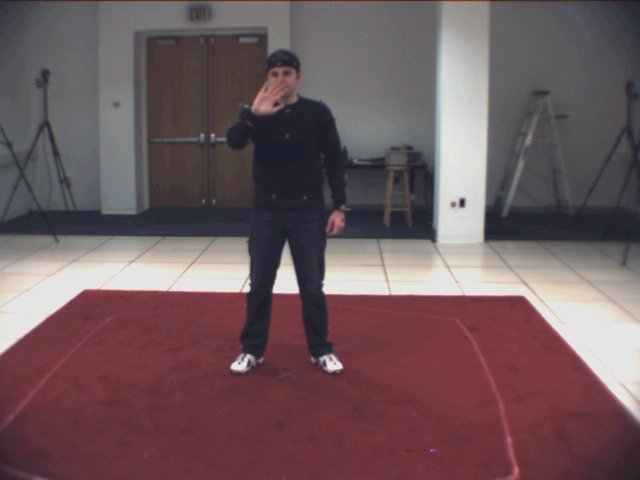
\includegraphics[height=6cm]{humaneva1.png}}
    \hspace{2cm}
    \subcaptionbox{输出}{
    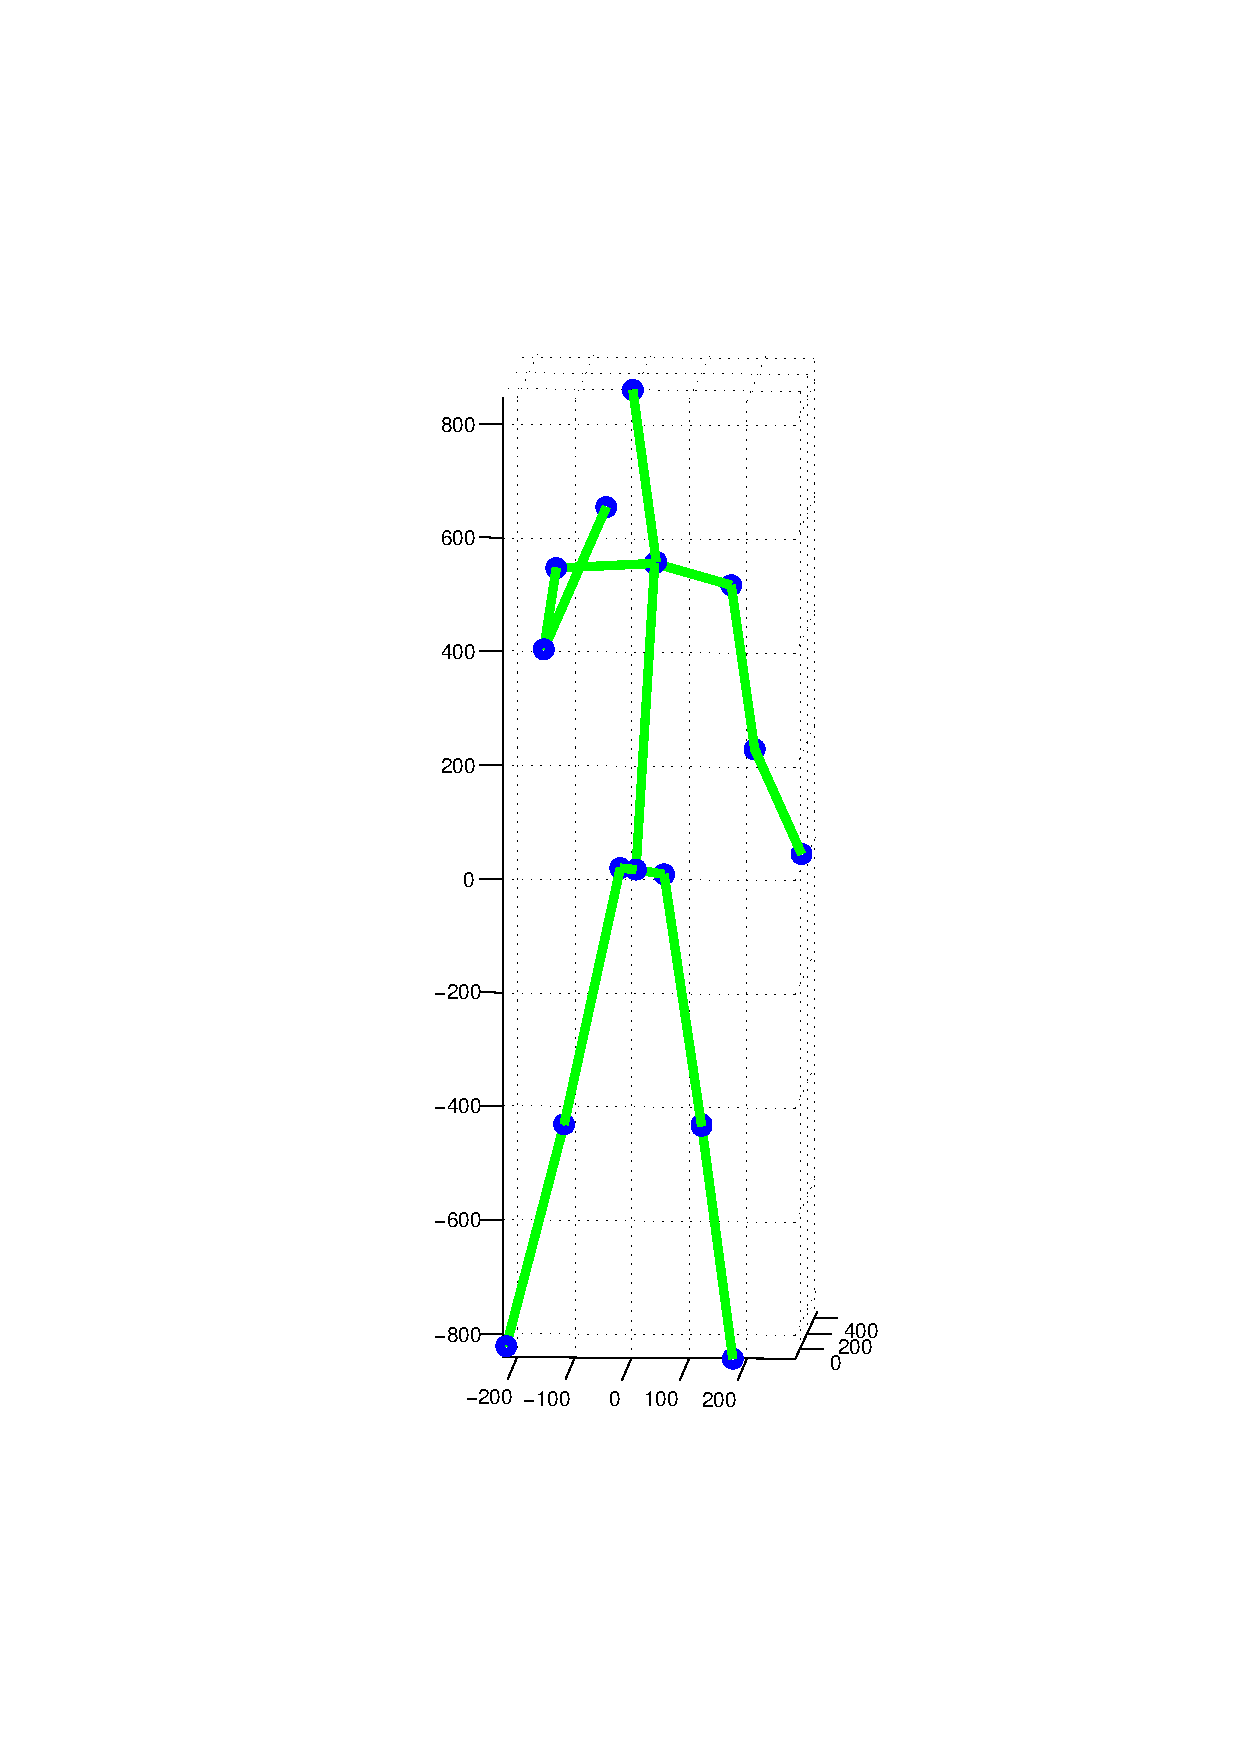
\includegraphics[height=6cm]{humaneva1_bone.pdf}}
    \caption{本文研究问题的输入与输出}
    \label{fig:inout}
\end{figure}


\section{文章结构}
本文共分为六章,第二章将介绍本人研究工作所依赖的数据库,包括数据库的内容、统计信息以及如何利用数据库等,其次介绍了本文所用的人体骨架模型的表示方法。第三章将介绍特征提取的一些方法,以及本文采用的特征以及其表示方法。第四章详细介绍了姿态估计算法,该算法基于双高斯过程,较好地考虑了输入输出变量之间的耦合关系。第五章主要以图表的方式整理了所做工作的结果,通过与前人工作对比,证明了本文工作的意义,并从结果中发现总结问题,分析可能的原因。第六章对全文做以总结,最后针对还存在的问题提出一些可能的解决方法和未来的努力方向。




\chapter{构建三维人体姿态数据库}
由于人体姿态估计算法大部分为监督学习,因此研究者制作了很多用于训练和测试的数据库,这些数据库有些是从互联网、电影中获得的图片,并人工标记出骨架作为ground-truth,有些是通过标记点或传感器等手段在拍摄影像的同时记录人体姿态的ground-truth。表\ref{tab:benchmark}整理了目前常用的人体数据库,本文采用了HumanEva-I~\cite{sigal2006humaneva}数据库,将在\ref{sec:HumanEva}节介绍。

\begin{table}[htbp]
  \centering
  \renewcommand{\arraystretch}{1.5}
  \begin{minipage}[t]{\linewidth} % 如果想在表格中使用脚注,minipage是个不错的办法
  \caption{常用姿态估计数据库汇总}
  \label{tab:benchmark}
    \begin{tabular}{c|p{7em}<{\centering}cp{6em}<{\centering}cp{5em}<{\centering}p{3em}<{\centering}}
      \toprule[1.5pt]
      \multicolumn{2}{c}{数据集} & 数据格式 & 说明 & 误差度量 & 帧数 & 复杂度 \\\midrule[1pt]
      \multirow{7}{1em}{\rotatebox{90}{单目二维}} & Agarwal/Triggs~\cite{agarwal20043d} & 图片 & 3D运动捕捉 & AJA\footnote{Average Joint Angel Error~\cite{agarwal20043d}~\cite{pons2010multisensor}} & 训练:1927 测试:418 & 简单\\
       & Buffy Stickmen~\cite{ferrari2008progressive} & 图片 & 2D上身姿势 & PCP\footnote{Percentage of Correctly Estimated Body Parts~\cite{ferrari2008progressive}~\cite{eth_biwi_00661}~\cite{tran2010improved}~\cite{ramanan2007learning}~\cite{Johnson10LSP}~\cite{yao2010modeling}} & 748 & 日常\\
       & ETHZ PASCAL Stickmen~\cite{eth_biwi_00661} & 图片 & 2D上身姿势 & PCP & 549 & 日常\\
       & UIUC Stickmen~\cite{tran2010improved} & 图片 & 2D上身姿势 & PCP & 训练:346 测试:247 & 日常\\
       & PARSE~\cite{ramanan2007learning} & 图片 & 2D完整姿势 & PCP & 训练:100 测试:205 & 复杂\\
       & Leeds Sports Poses Dataset~\cite{Johnson10LSP} & 图片 & 2D完整姿势 & PCP & 训练:1000 测试:1000 & 复杂\\
       & Human-Object Interaction~\cite{yao2010modeling} & 图片 & 2D完整姿势\ 2D运动 & PCP & 训练:180 测试:120 & 复杂\\\midrule[0.5pt]
      \multirow{3}{1em}{\rotatebox{90}{多目三维}} & HumanEva~\cite{sigal2006humaneva} & 多目视频 & 三维运动捕捉 & AJP\footnote{Average Joint Position Error~\cite{ganapathi2010real}~\cite{sigal2006humaneva}~\cite{wang2006modular}} & 约80000 & 日常\\
      & MPI08~\cite{pons2010multisensor} & 多目视频 & 内部传感器\ 三维激光扫描 & AJA & 约24000 & 日常\ 复杂\\
      & Stanford ToF~\cite{ganapathi2010real} & ToF 深度 & 三维运动捕捉 三维激光扫描 & AMP\footnote{Average Marker Position Error} & 27 个序列 & 日常\ 复杂\\
      \bottomrule[1.5pt]
    \end{tabular}
    \end{minipage}
\end{table}

\section{HumanEva数据库}
\label{sec:HumanEva}
由于本文所做工作为人体三维姿态估计,不仅需要多个视角的视频数据,还需要对人物进行运动捕捉,记录关节点的位置,这项工作十分繁琐,由于经历和时间有限,也为了能和已有算法进行更好对比,最后选择了HumanEva数据库作为训练和测试的依据。
\subsection{数据来源}
尽管近年来姿态估计的算法百花齐放,但是由于不同算法基于不同的数据库,度量标准也有所差别,而且很多数据只是二维图片和骨架,缺少三维骨架信息,因此算法能利用的数据库十分有限,且不同算法之间很难比较,为了解决如上问题,美国布朗大学于2006年在本田研究所和英特尔公司的支持下设计制作了HumanEva数据库。该数据库用多台相机同步记录了多视点的人体动作视频,并用运动捕捉的方法记录了三维姿态信息,同时各相机也进行了标定,因此也可以计算得到二维姿态信息,在给出数据本身的同时,项目组还为姿态估计领域的研究者提供了一个简单的示例程序,演示了如何读取数据库,此外项目组还给出了一套计算误差的标准和网络提交平台,供研究者上传自己的算法结果,与他人结果进行对比。因此,该数据库的出现,不仅让研究者有了易用的大量数据,而且促进了该领域的交流与发展。

\subsection{数据统计}
HumanEva数据库一共包含两部分,分别为HumanEva-I和HumanEva-II,I代表数据制作的批次,两者的区别见表~\ref{tab:I-II}。本文采用的是HumanEva-I,用七台同步相机以每秒60帧的速度记录了四位演员分别表现的六种动作,共计13.5G视频资料,具体数据详见表\ref{tab:totalframes},相机的摆放位置参照图\ref{fig:camera},图\ref{fig:demo} 展示了数据库的样例。
\begin{table}[htbp]
  \centering
  \caption{HumanEva-I vs HumanEva-II}
  \label{tab:I-II}
    \begin{tabular}{lcc}
      \toprule[1.5pt]
       & HumanEva-I & HumanEva-II \\\midrule[1pt]
      同步方式 & 软件 & 硬件\\
      相机数量 & 7 & 4\\
      相机种类 & 3彩色+4黑白 & 4彩色\\
      运动捕捉相机数 & 6 & 8\\
      数据类别 & 训练、验证、测试 & 测试\\
      \bottomrule[1.5pt]
    \end{tabular}
\end{table}

\begin{table}[htbp]
  \centering
  \caption{HumanEva-I训练+验证帧数统计}
  \label{tab:totalframes}
    \begin{tabular}{lcccc}
      \toprule[1.5pt]
      动作 & Subject1 & Subject2 & Subject3 & 合计 \\\midrule[1pt]
      走路 & 1315 & 1047 & 1020 & 3382 \\
      慢跑 & 820 & 952 & 908 & 2680 \\
      投掷 & 1052 & 1256 & 1111 & 3419 \\
      挥手 & 872 & 1052 & 1199 & 3123 \\
      拳击 & 863 & 916 & 1084 & 2863 \\
      合计 & 4922 & 5223 & 5322 & 15467\\
      \bottomrule[1.5pt]
    \end{tabular}
\end{table}

\begin{figure}[htbp]
  \centering
  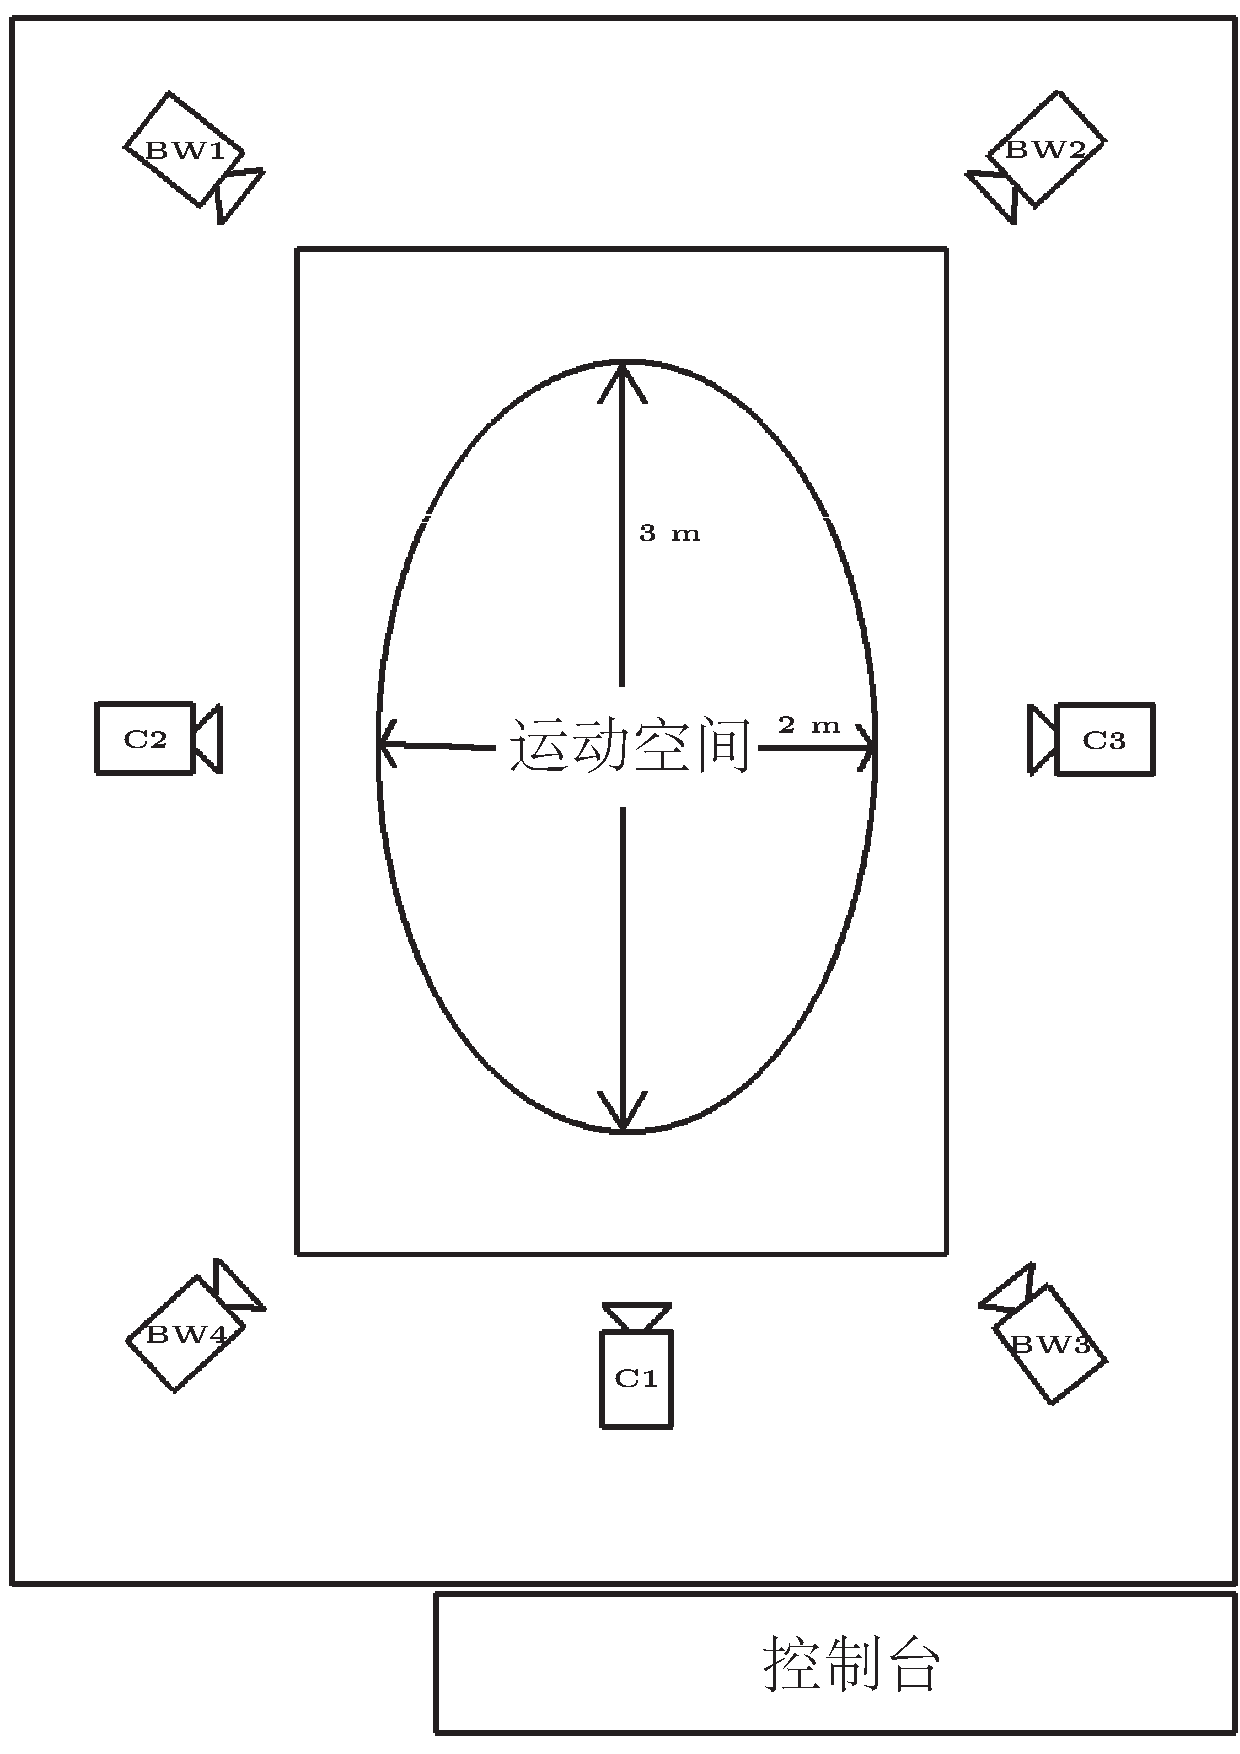
\includegraphics[height=8cm]{camera.pdf}\\
  \caption{相机摆放位置}\label{fig:camera}
\end{figure}

\begin{figure}[htbp]
  \centering
  \subcaptionbox{S1}{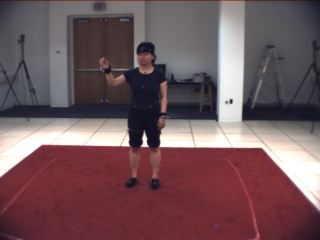
\includegraphics[width=0.4\textwidth]{S1}}\hspace{.5cm}
  \subcaptionbox{S2}{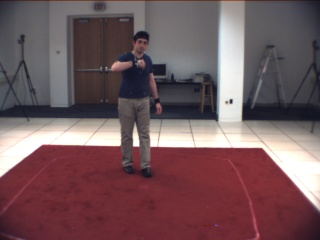
\includegraphics[width=0.4\textwidth]{S2}}\\
  \subcaptionbox{S3}{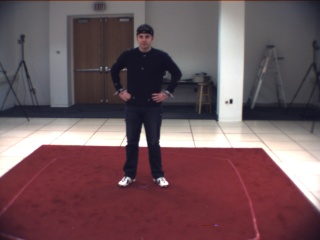
\includegraphics[width=0.4\textwidth]{S3}}\hspace{.5cm}
  \subcaptionbox{S4}{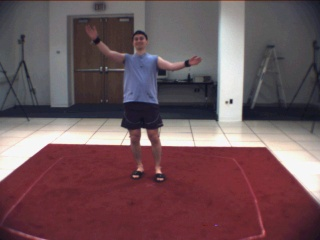
\includegraphics[width=0.4\textwidth]{S4}}
  \caption{HumanEva-I样例}\label{fig:demo}
\end{figure}

然而,数据库只对部分视频资料给出了运动姿态的ground-truth,四号演员的所有视频都只能用来测试,一到三号演员也有一半视频都没有ground-truth。此外,由于运动捕捉系统本身的问题,并不是对所有视频帧都能给出正确的三维姿态,因此经过筛选后\cite{Poppe2007}\cite{bo2010twin}文章所使用的训练数据如表\ref{tab:poppe}所示。在本文中,训练使用的帧数比\cite{Poppe2007}\cite{bo2010twin}文章较多,具体见表\ref{tab:mydataset}。

\begin{table}[htbp]
  \centering
  \caption{\cite{Poppe2007}\cite{bo2010twin}文章所用帧数统计}
  \label{tab:poppe}
    \begin{tabular}{lcccc}
      \toprule[1.5pt]
      动作 & Subject1 & Subject2 & Subject3 & Total \\\midrule[1pt]
      走路 & 1176 & 876 & 895 & 2947 \\
      慢跑 & 439 & 795 & 831 & 2065 \\
      投掷 & 217 & 806 & 0 & 1023\\
      挥手 & 801 & 681 & 214 & 1696\\
      拳击 & 502 & 464 & 933 & 1889\\
      合计 & 3135 & 3622 & 2873 & 9630\\
      \bottomrule[1.5pt]
    \end{tabular}
\end{table}

\begin{table}[htbp]
  \centering
  \caption{本文所用帧数统计}
  \label{tab:mydataset}
    \begin{tabular}{lcccc}
      \toprule[1.5pt]
      动作 & Subject1 & Subject2 & Subject3 & Total \\\midrule[1pt]
      走路 & 1220 & 913 & 976 & 3109 \\
      慢跑 & 506 & 824 & 897 & 2227 \\
      投掷 & 217 & 815 & 0 & 1032\\
      挥手 & 872 & 690 & 260 & 1822\\
      拳击 & 576 & 470 & 996 & 2042\\
      合计 & 3391 & 3712 & 3129 & 10232\\
      \bottomrule[1.5pt]
    \end{tabular}
\end{table}



\section{人体三维骨架表示}
\label{sec:skeleton}

本文采用的人体三维骨架表示方法同\cite{bo2010twin},将人体用20个关节点来描述,每个关节点用$\mathbf{P}=(x,y,z)$三维坐标表示,串联起来构成$20\times3=60$维向量。在二维图像上表示骨架如图\ref{fig:2Ddemo},三维表示如图\ref{fig:3Ddemo},20个关节点的具体含义参见表\ref{tab:20}。为了使每个骨架对齐,我们把躯干远端作为三维坐标的原点,所有其他点坐标都根据原点做平移变换。

\begin{figure}[htbp]
  \centering
  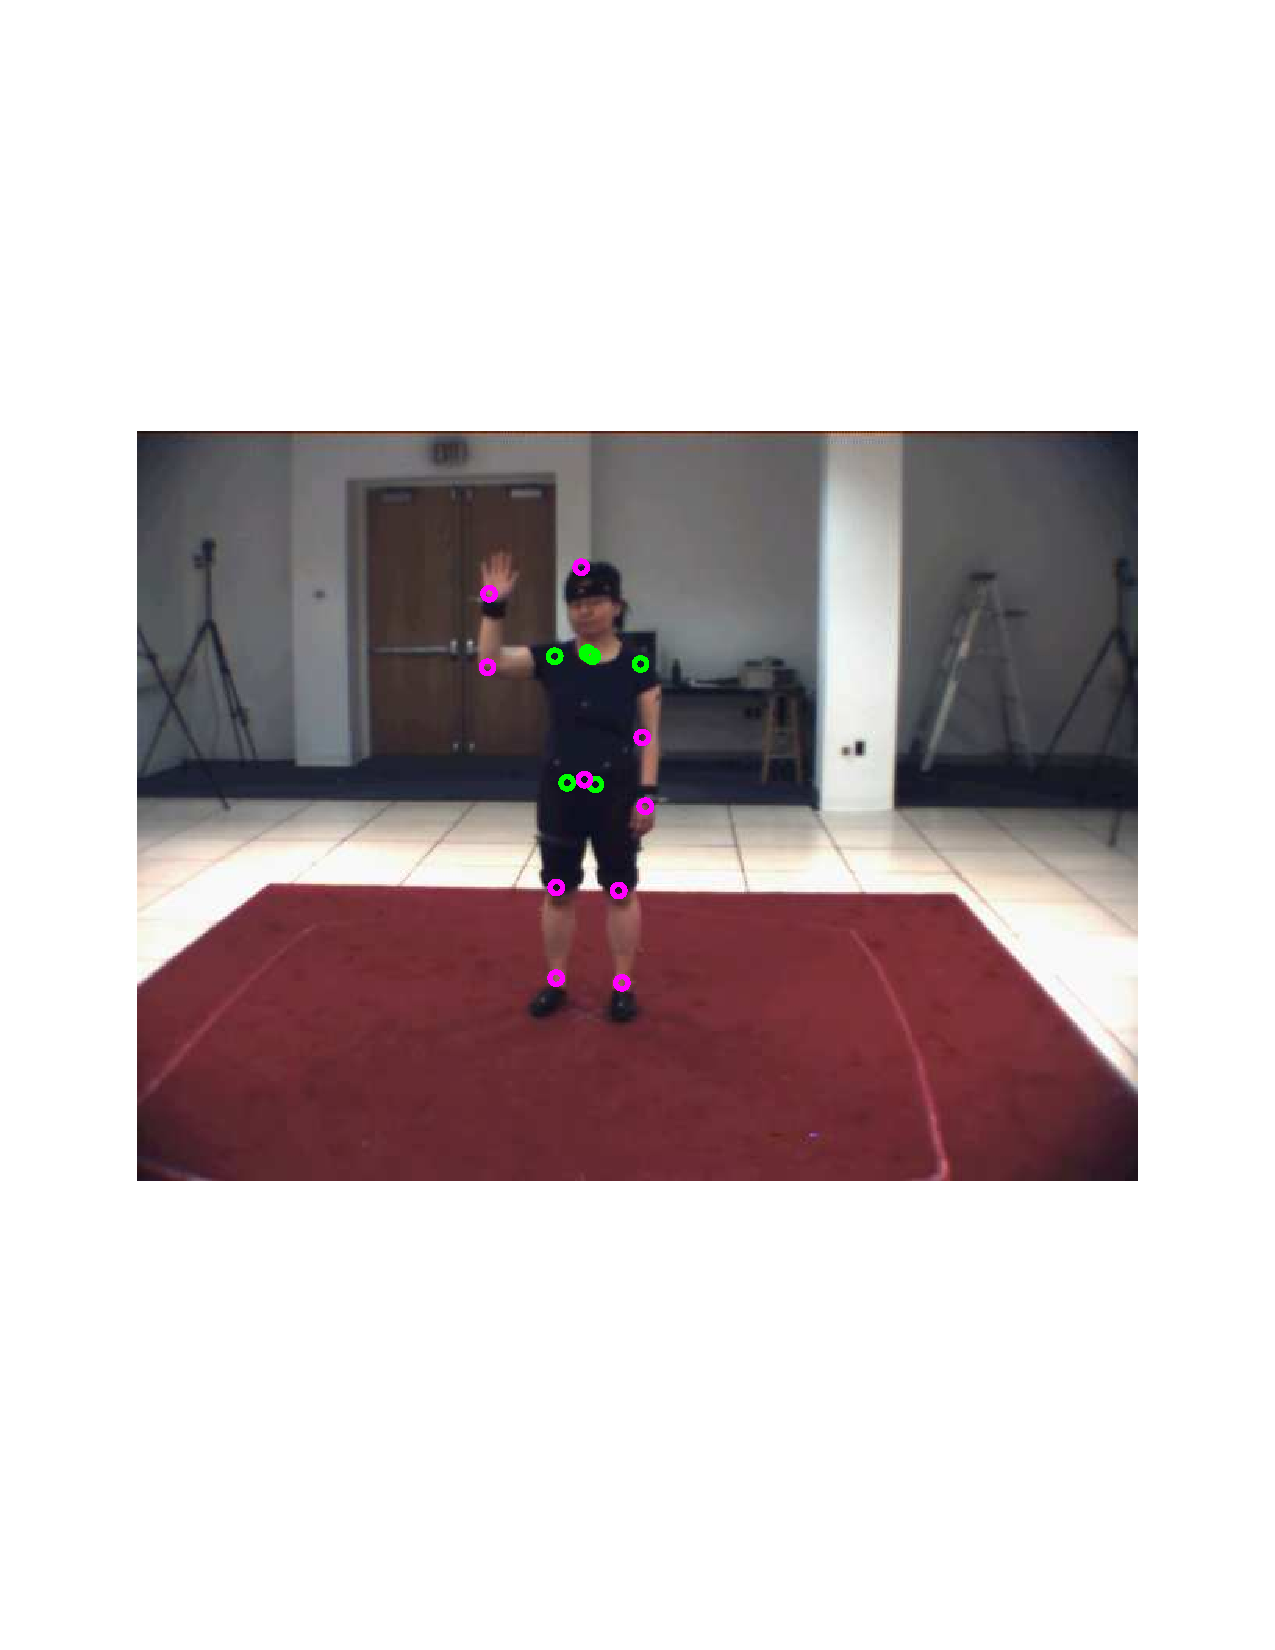
\includegraphics[width=0.7\textwidth]{2Dpose}\\
  \caption{二维骨架表示}\label{fig:2Ddemo}
\end{figure}

\begin{figure}[htbp]
  \centering
  \subcaptionbox{}{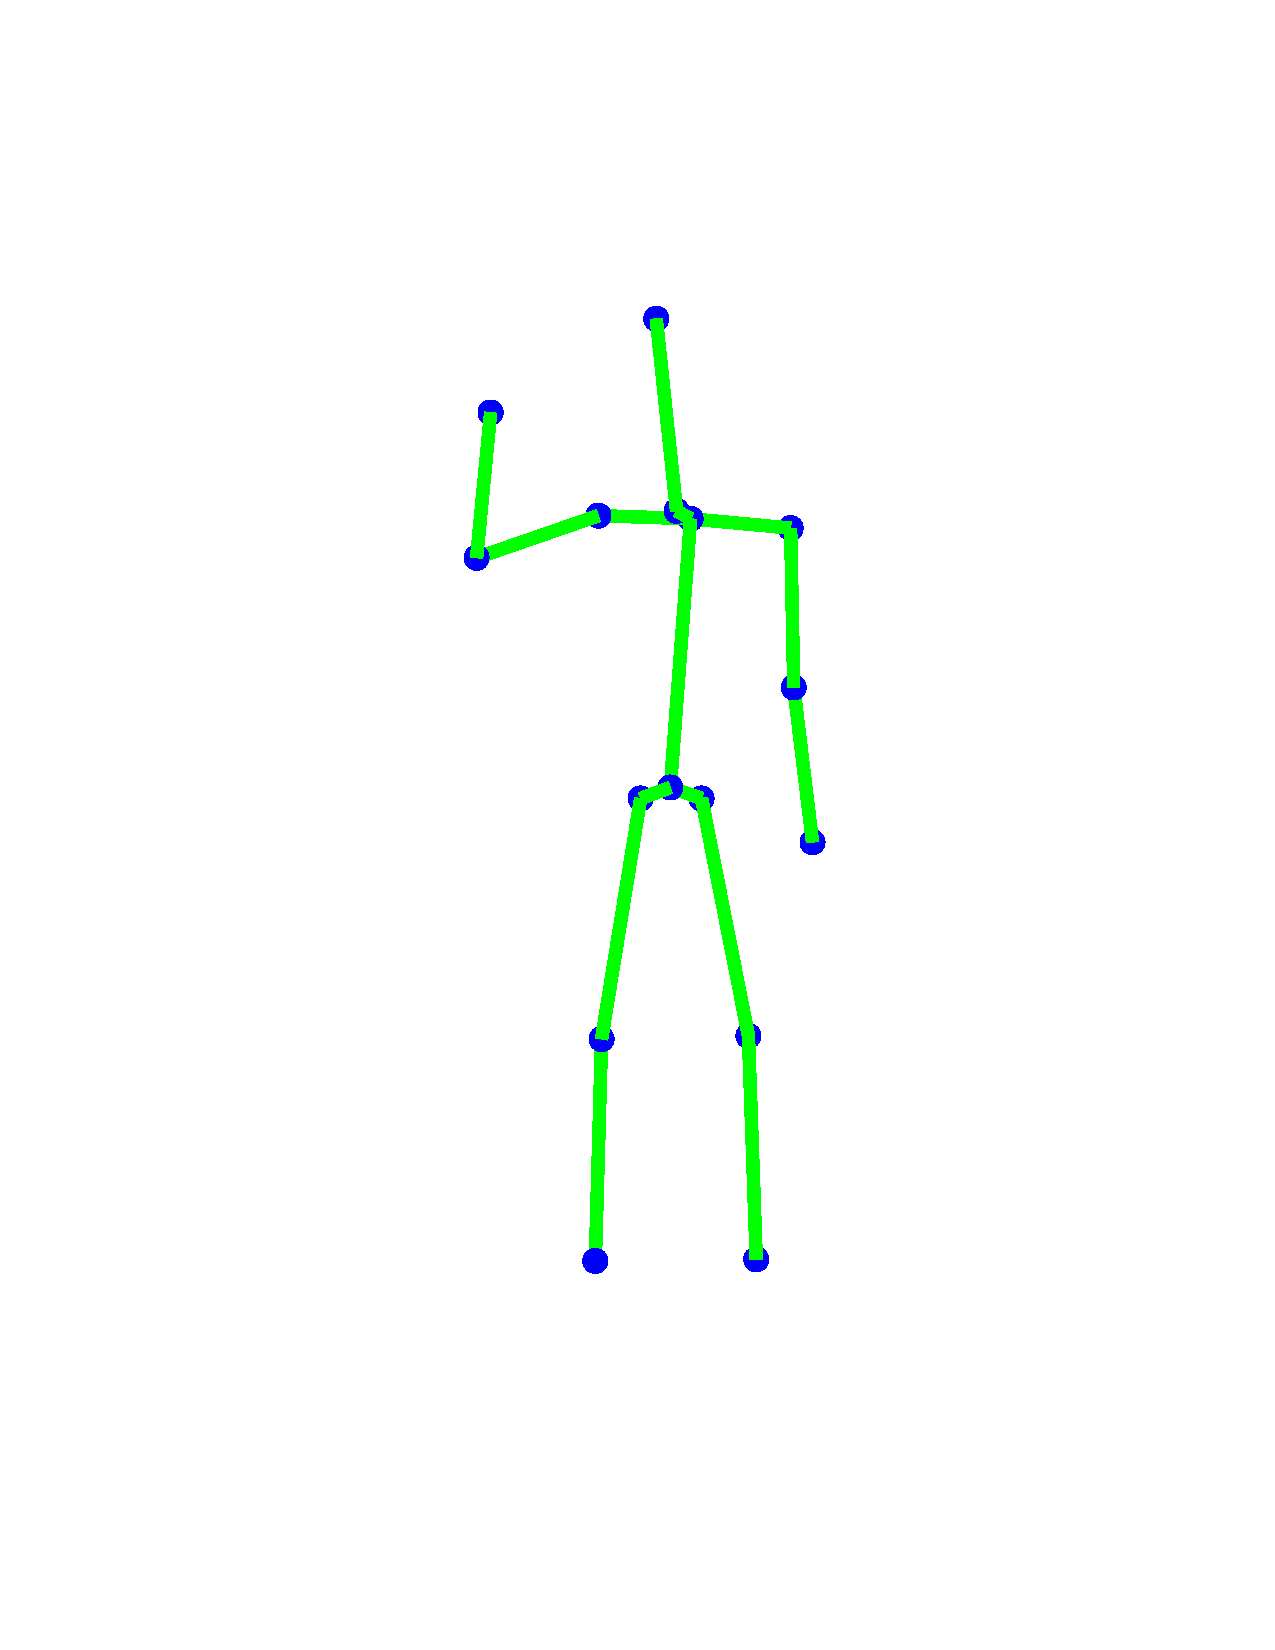
\includegraphics[height=6cm]{3D_1}}\hspace{1cm}
  \subcaptionbox{}{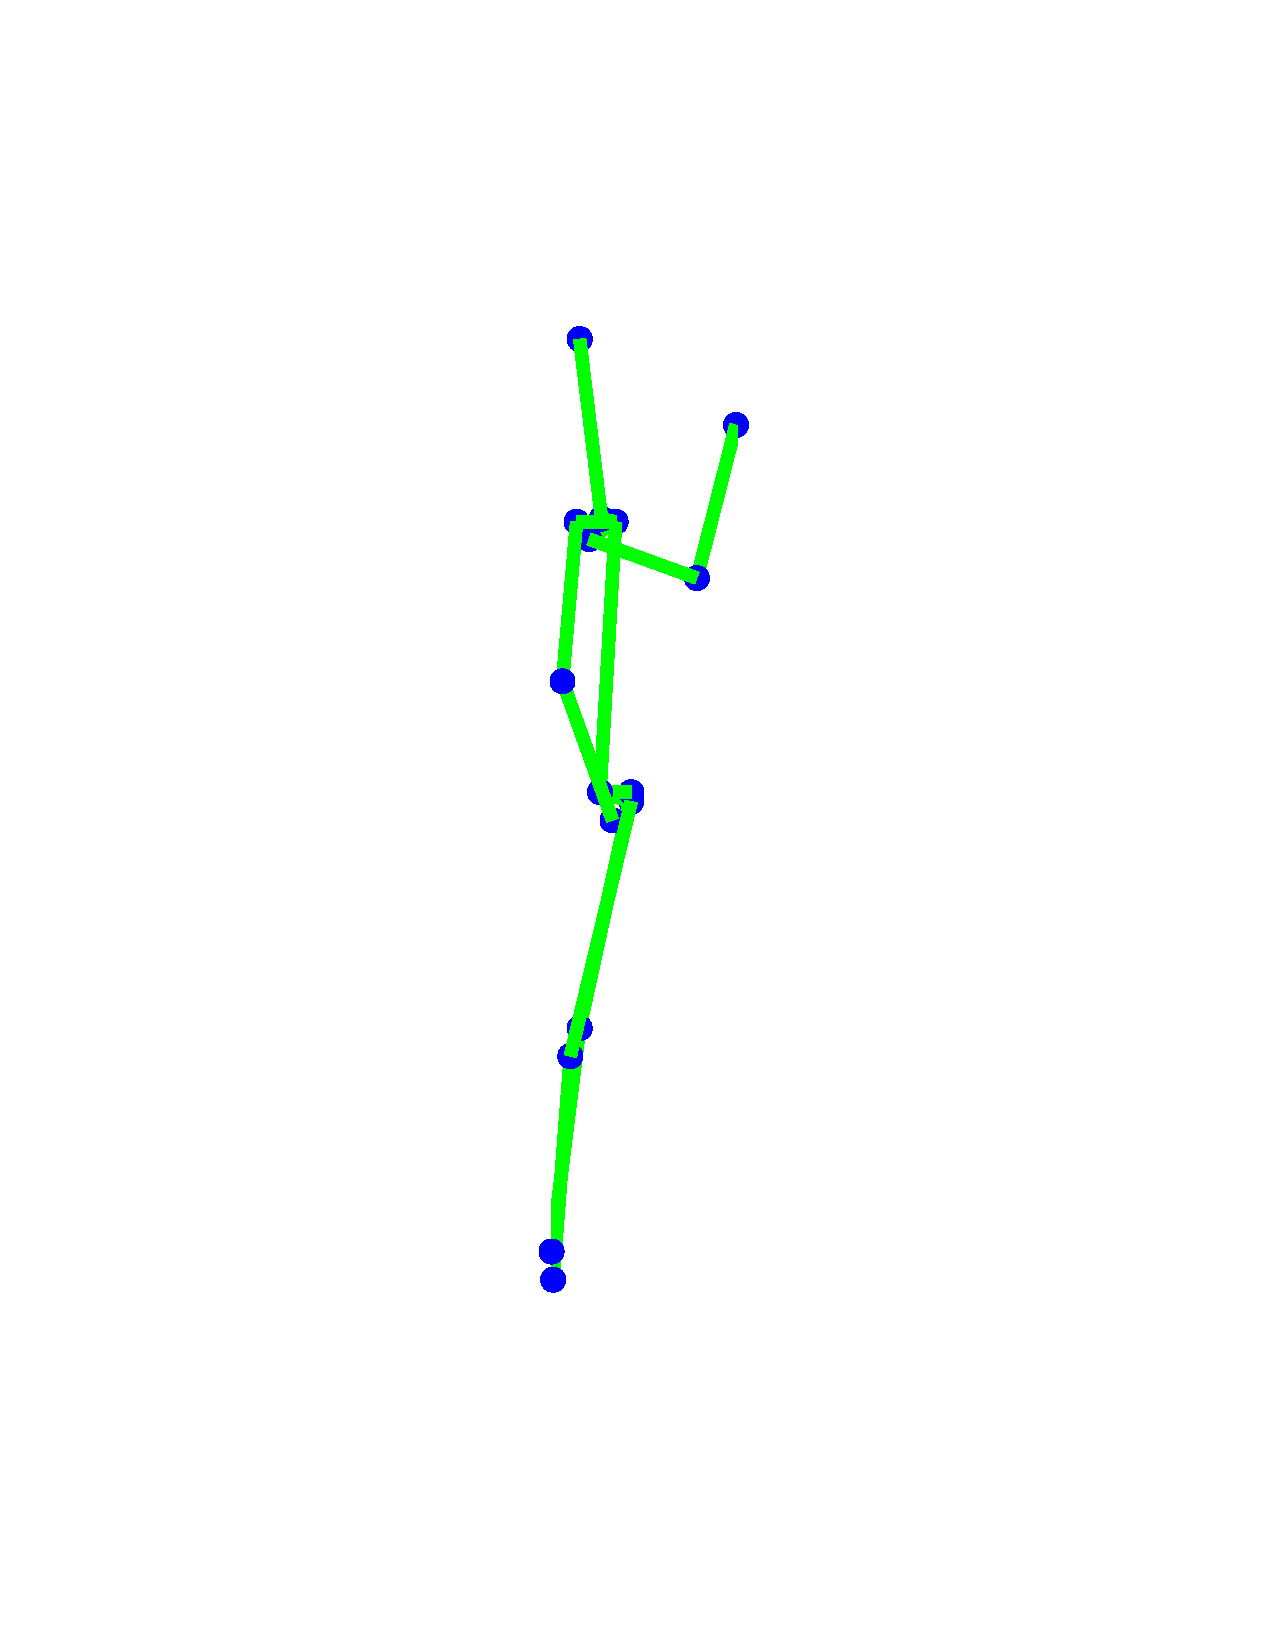
\includegraphics[height=6cm]{3D_2}}\hspace{1cm}
  \subcaptionbox{}{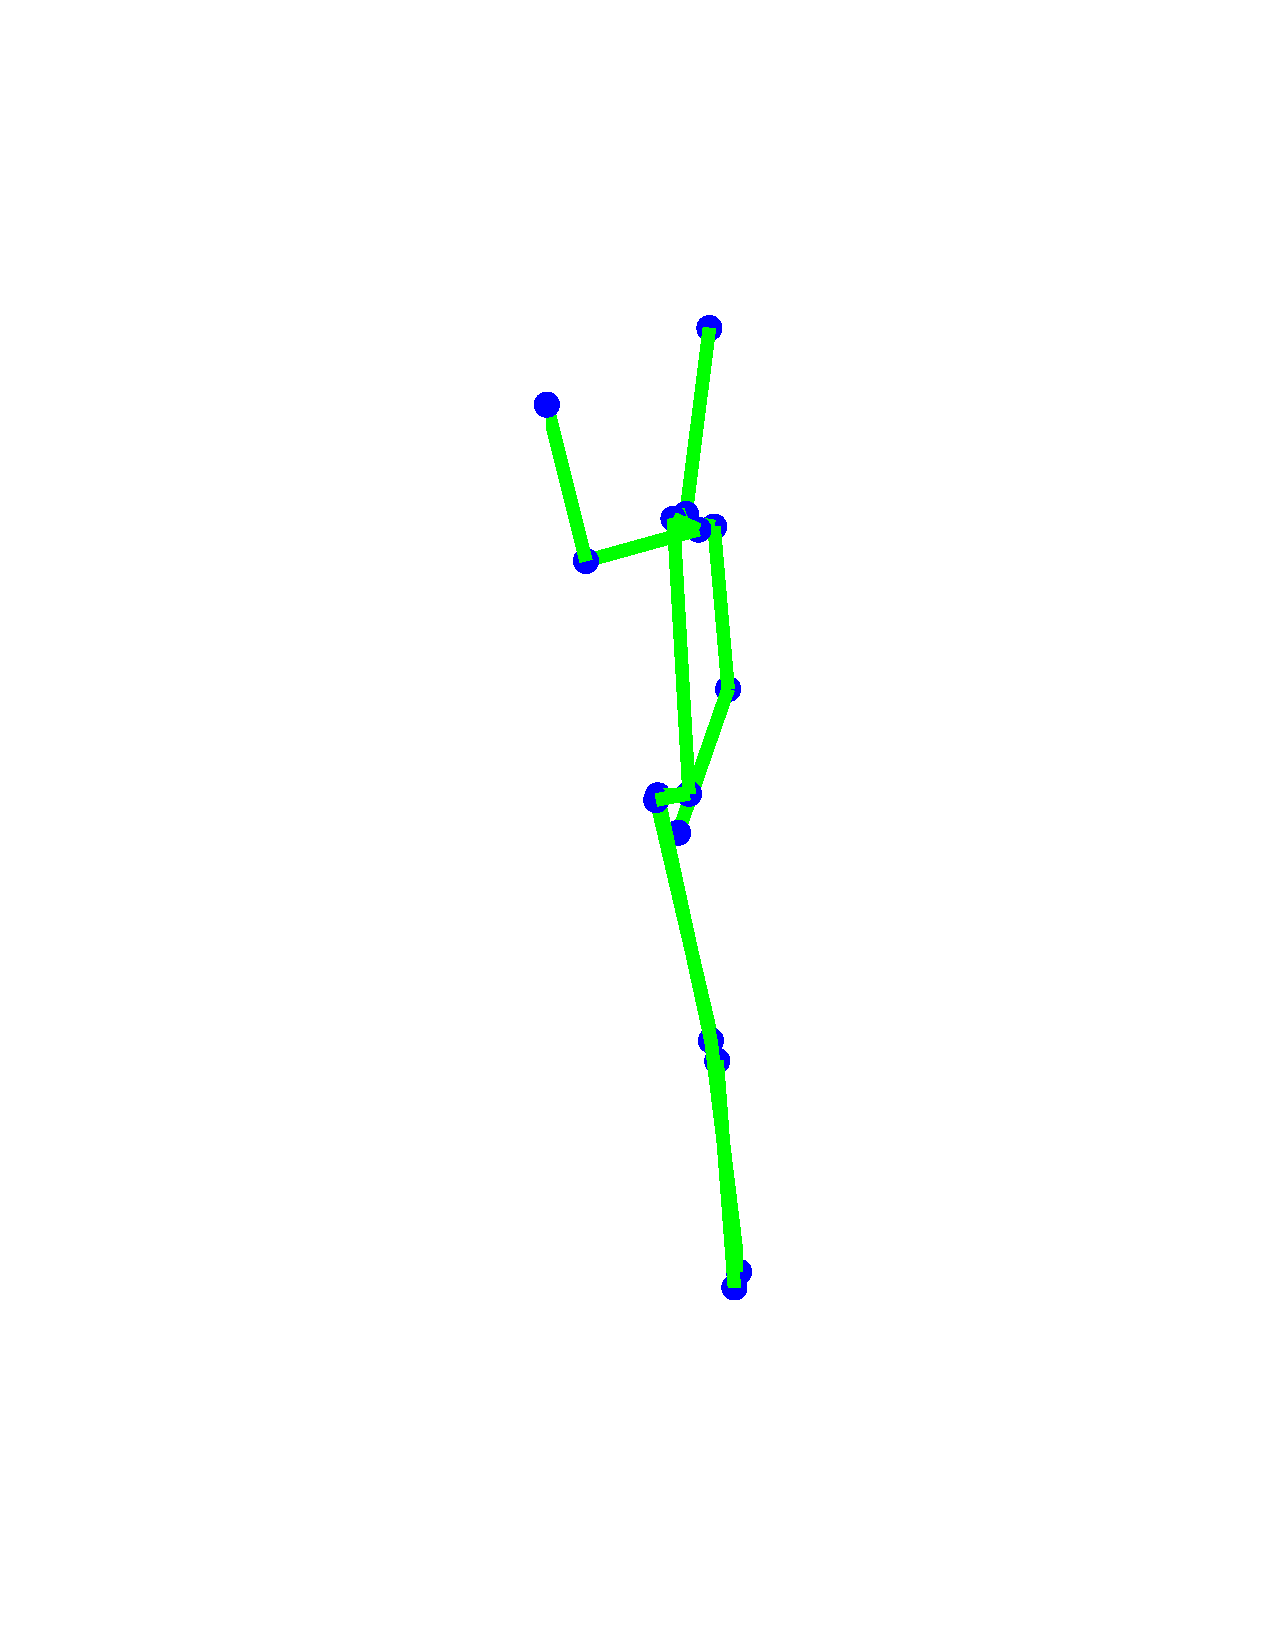
\includegraphics[height=6cm]{3D_3}}
  \caption{三维骨架表示}\label{fig:3Ddemo}
\end{figure}

\begin{table}[htbp]
  \centering
  \begin{tabular}{ccccccccccc}
  \toprule[1.5pt]
    & \multirow{2}{4em}{躯干}  & \multirow{2}{4em}{头部}  & \multicolumn{4}{c}{胳膊} & \multicolumn{4}{c}{腿}\\
    & & & 左前 & 左后 & 右前 & 右后 & 左前 & 左后 & 右前 & 右后 \\\midrule[1pt]
   近端 & 1 & 1 & 1 & 1 & 1 & 1 & 1 & 1 & 1 & 1 \\
   远端 & 1 & 1 & 1 & 1 & 1 & 1 & 1 & 1 & 1 & 1 \\
   \bottomrule[1.5pt]
  \end{tabular}
  \caption{关节点构成}\label{tab:20}
\end{table}



\chapter{提取特征}
\label{chap:feature}
本文采用的是基于特征的方法,如何用合适的特征描述图像显得至关重要。首先,选取的特征需要能很好地刻画人物的姿态信息,即相似姿态具有相似的特征,不同姿态的特征的区别也要足够明显,尽可能让特征只包含姿态信息,不会因为光照、图片尺寸、衣服、人物体型的改变受到剧烈变化。其次,特征的维数不能太高,否则会增加学习和预测过程中的计算量。同时提取特征本身的计算量也要加以限制。
经过调查发现,目前最好的姿态估计算法~\cite{ramanan2007learning}~\cite{yang2011articulated}~\cite{tian2012exploring} 大都采用了HOG(Histogram of Oriented Gradient,方向梯度直方图)的特征,也有一些文献采用了其他的特征,如\cite{bo2008fast}采用了SIFT(scale-invariant feature transform)和HistoSC(Histogram of Shape Context)的特征,\cite{eth_biwi_01027}采用了Lab颜色空间统计和皮肤检测的特征,本文同多数算法一样采用了HOG特征,并做了一些改进,此外,还提出了一种能表示皮肤信息的特征,取得了较好的结果。
\section{图片预处理}
为了剔除环境对提取特征的影响,在提取特征前首先要提取ROI(Region Of Interests)。在本文中,ROI即为图片中的人物,提取ROI即背景分离,任务是把人物从图片中分割出来,并裁剪图片。由图\ref{fig:demo}可以看出HumanEva数据库的环境是非常复杂的,好在数据库提供了纯背景的图像序列\ref{fig:background},因此可以在已知背景情况下分割人物。尽管这项任务是计算机视觉领域中一个非常久远且已经攻克的问题,但由于这不是本文重点,因此没有花太多时间和精力调查文献和实现算法,本文用一系列简单的操作实现了比\cite{Poppe2007}更好的分割效果。
\begin{figure}[htbp]
  \centering
  \subcaptionbox{C1}{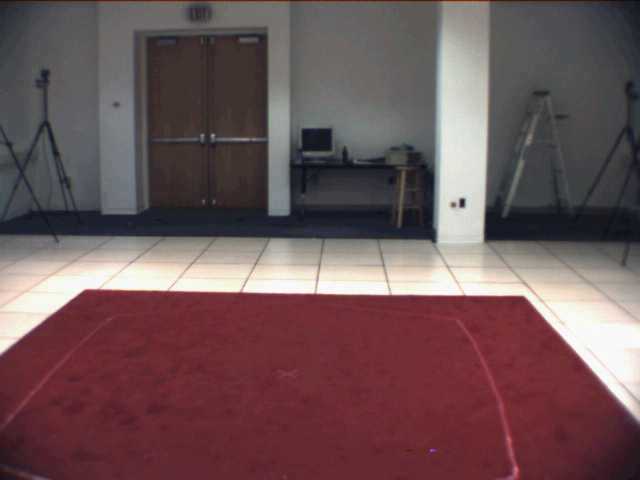
\includegraphics[width=0.31\textwidth]{bk_C1}}
  \subcaptionbox{C2}{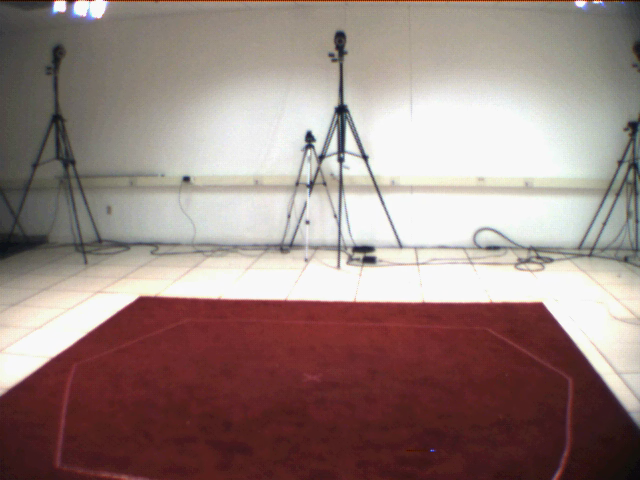
\includegraphics[width=0.31\textwidth]{bk_C2}}
  \subcaptionbox{C3}{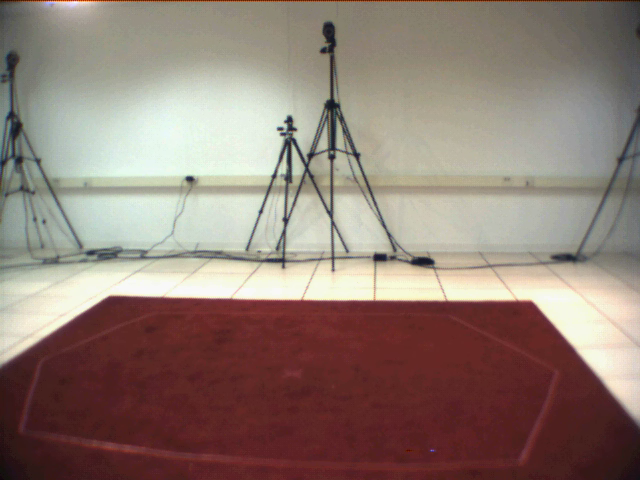
\includegraphics[width=0.31\textwidth]{bk_C3}}
  \caption{HumanEva背景}\label{fig:background}
\end{figure}
\subsection{计算背景数据}
给出的背景不是单张图片,而是一段视频,因此可利用的信息更多。本文假定视频中的$N$帧图像每个像素点都满足高斯分布,记像素点$\mathbf{c}=(r,g,b)$,则$\mathbf{c}\sim \mathcal{N}(\mu,\sigma)$,通过统计所有视频帧可以算出$\mu$和$\sigma$,用待分割图片中的每一个像素点代入高斯分布,即可算出该点是否为背景的概率。给定一个阈值,即可产生一个粗糙的二值图分割,见图\ref{fig:bk1}。
\begin{figure}[htbp]
  \centering
  \subcaptionbox{原图}{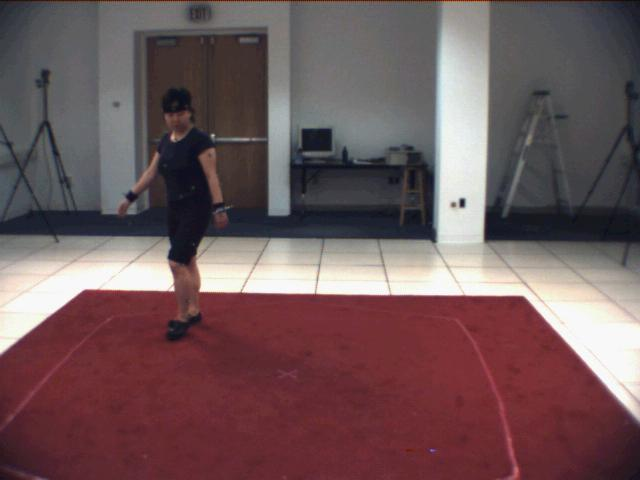
\includegraphics[width=0.45\textwidth]{bkimage}}\hspace{.5cm}
  \subcaptionbox{背景概率分割}{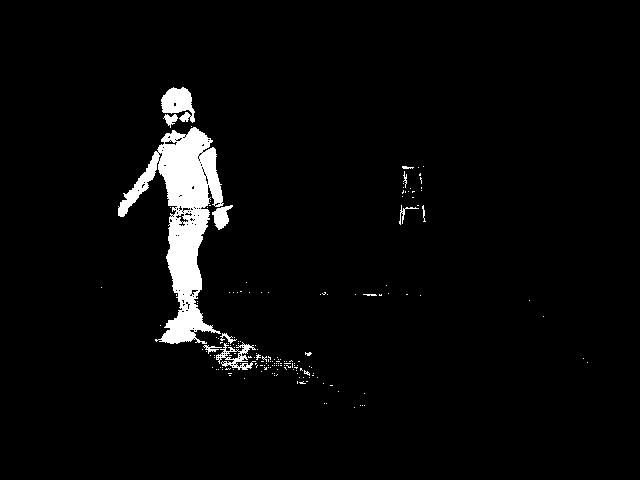
\includegraphics[width=0.45\textwidth]{bk1}}
  \caption{HumanEva背景分割1}\label{fig:bk1}
\end{figure}

\subsection{局部优化}
可以看出,用简单的阈值分割无法保证正确性,部分背景被认为是前景(即所需人物),而前景中夹杂的与背景相似的颜色(尤其是脸部,和背景中的门颜色过于相近,残缺很多)则被认为是背景,于是又做了很多优化。首先,需要把明显不是前景的背景去掉,这里考虑用距离来度量,即偏离人物较远的均认为是背景。具体做法是先找到图中最大面积区域的位置,该区域被近似为前景位置,将偏离该区域较远的区域都认为是背景(因为数据库中人物的动作范围不大,长宽均有限,这里把阈值选为80 像素),可以从图\ref{fig:bkfar}看出偏远大块的背景已经被去掉。

\begin{figure}[htbp]
  \centering
  \subcaptionbox{}{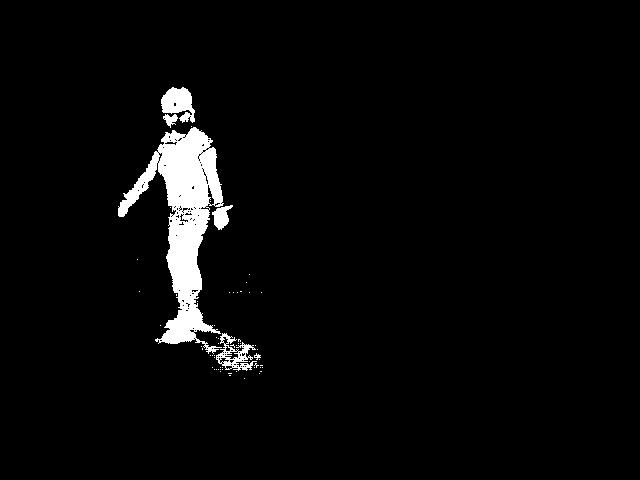
\includegraphics[height=5.5cm]{bkfar}}\hspace{1cm}
  \subcaptionbox{}{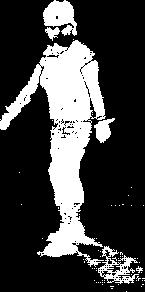
\includegraphics[height=5.5cm]{bkfarcut}}
  \caption{HumanEva背景分割2}\label{fig:bkfar}
\end{figure}

然而由于人物遮挡光线产生的阴影还存在,因此需要考虑去掉人物产生的阴影。去除阴影用了最简单的方法,即把原图先裁剪至最小前景区域,只考虑该区域底部20\%的区域,将这小部分区域转换到HSV颜色空间,同样在纯背景中对相同区域做HSV变换,仅对色相通道做差,手工选定阈值,再与已有分割对应部分做与运算,即可将阴影去除,阴影去除后的效果见图\ref{fig:bk2foot}。

\begin{figure}[htbp]
  \centering
  \subcaptionbox{原图}{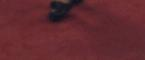
\includegraphics[width=0.3\textwidth]{bkfootorg}}\hspace{.5cm}
  \subcaptionbox{背景}{
\includegraphics[width=0.3\textwidth]{bkfootbk}}\\
  \subcaptionbox{原图HSV}{
\includegraphics[width=0.3\textwidth]{bkfootorghsv}}\hspace{.5cm}
  \subcaptionbox{背景HSV}{
\includegraphics[width=0.3\textwidth]{bkfootbkhsv}}\\
  \subcaptionbox{做差}{
\includegraphics[width=0.3\textwidth]{bkfootdiff}}\\
  \caption{去除阴影}
\end{figure}

此时还有一些背景噪音,接着去掉了前景中面积较小的部分,面积的阈值可以选的小一些,在这里选择为40像素(图像为$480\times 640$像素),这些部分大多都是未能剔除的环境噪音,此时结果参见图\ref{fig:bk3small}。

\begin{figure}[htbp]
  \centering
  \subcaptionbox{去除阴影\label{fig:bk2foot}}{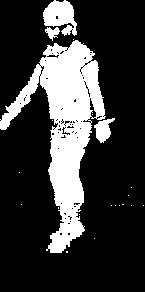
\includegraphics[height=5.5cm]{bkshadowrem}}\hspace{1cm}
  \subcaptionbox{去掉小块背景\label{fig:bk3small}}{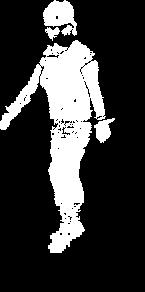
\includegraphics[height=5.5cm]{bksmall1}}
  \caption{HumanEva背景分割3}
\end{figure}

由于人物的脸部等地方有较大缺失,于是接着做了8次膨胀\footnote{在膨胀前先对图像加框,防止越界}(半径为1的圆形,见图\ref{fig:bk4dilate}),和8次腐蚀(同样半径为1,见图\ref{fig:bk4erode}),最后做一次背景抹除(面积小于400像素的都被消去),此时只剩下了单一连通的前景。

\begin{figure}[htbp]
  \centering
  \subcaptionbox{膨胀\label{fig:bk4dilate}}{
\includegraphics[height=5.5cm]{bkdilate}}\hspace{1cm}
  \subcaptionbox{腐蚀\label{fig:bk4erode}}{
\includegraphics[height=5.5cm]{bkerode}}
  \caption{HumanEva背景分割4}
\end{figure}

与\cite{Poppe2007}对比可以看出,该文献的前景(见图\ref{fig:bk_cmp_org})有较多空洞,这对于HoG的计算会带来很大误差,而本文提出的分割方法(见图\ref{fig:bk_cmp_my})没有小块噪音,整个前景连为一体,虽然在边缘轮廓不是特别准确,但是对于HoG特征来说影响不大。

\begin{figure}[htbp]
  \centering
  \subcaptionbox{Poppe等人分割结果\label{fig:bk_cmp_org}}{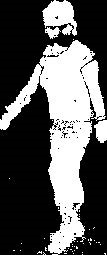
\includegraphics[height=5.5cm]{bk_cmp_org}}\hspace{1cm}
  \subcaptionbox{本文结果1\label{fig:bk_cmp_my}}{
\includegraphics[height=5.5cm]{bk_cmp_my}}\hspace{1cm}
  \subcaptionbox{本文结果2\label{fig:bk_cmp_my2}}{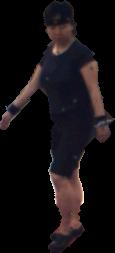
\includegraphics[height=5.5cm]{bk_final}}
  \caption{背景分割对比}
\end{figure}

此外,在处理演员2的时候由于衣服颜色和背景过于相像,出现了图\ref{fig:bkerr} 所示的错误(上身部分缺失),针对这种特殊情况,先找到前景所占矩形区域,然后填充矩形区域中上部60\%范围内的空洞。这一操作虽然不至于填充两腿缝隙,但对于胳膊与腰造成的空洞也会一并填充,鉴于这种情况出现的帧数极少,故忽略此问题。

\begin{figure}[htbp]
  \centering
  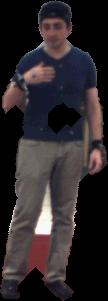
\includegraphics[height=5.5cm]{bkerr1}
  \caption{背景分割错误}\label{fig:bkerr}
\end{figure}

\section{HOG特征}
\subsection{概述}
HOG特征最早由Navneet Dalal和Bill Triggs在2005年提出~\cite{Dalal05histogramsof},被成功地用于目标检测,尤其是行人检测。该方法是对图像的局部区域出现的方向梯度进行统计,和SIFT相似,不同的是HOG用了重叠的局部对比度归一化(overlapping local contrast normalization)技术。HOG描述子的主要贡献是很好地描述了局部区域的边缘方向密度。对图像进行归一化后,能够很好地保证照射和阴影不变性。与其他方法相比,HOG有很好的几何和光学转化不变性,因此十分适合行人检测和姿态估计。
\subsection{计算HOG描述子}
HOG特征的提取方法主要步骤如下:
\begin{enumerate}
  \item 转化为灰度图像
  \item 划分成若干元胞(cell)
  \item 计算每个像素的梯度
  \item 统计每个子区域内梯度直方图
\end{enumerate}

具体说来,本文将$r,g,b$三个通道认为是三张灰度图,分别求取HOG特征,最后取每一维最大值,最后做归一化处理。伪代码见代码\ref{alg:maxhog}。
\newcommand{\comment}{\textbackslash\textbackslash}
\begin{algorithm}
  \caption{MAX-HOG}\label{alg:maxhog}
  \begin{algorithmic}[1]

    \FOR{$i=0$ to $image.NumberOfChannels$}
        \STATE H($i$) $\leftarrow$ GetHOG($image.channel(i)$);
    \ENDFOR

    \STATE  H $\leftarrow$ MAX(H($i$));
    \STATE  H $\leftarrow$ L1Norm(H);
    \RETURN H
  \end{algorithmic}
\end{algorithm}

针对每一张灰度图求取HOG特征的算法伪代码见代码\ref{alg:gethog}。

\begin{algorithm}
  \caption{GetHOG}\label{alg:gethog}
  \begin{algorithmic}[1]
    \STATE \comment 设置元胞数量,横向6个,纵向9个
    \STATE $Cell\_Num\_x \leftarrow 6;$
    \STATE $Cell\_Num\_y \leftarrow 9;$
    \STATE \comment 计算梯度\\
    \STATE $grad_x \leftarrow$ CalGrad$(image,hx)$;
    \STATE $grad_y \leftarrow$ CalGrad$(image,hy)$;
    \STATE $angle \leftarrow$ GetAngle$(grad_x,grad_y)$;\comment 计算梯度方向
    \STATE $magnit \leftarrow \sqrt(grad_yu^2+grad_xr^2)$;\comment 计算梯度大小
    \STATE \comment 计算直方图
    \FOR{$i=1$ to $Cell\_Num\_x\times Cell\_Num\_y$}
        \FOR{$j=0$ to 180, interval=20}
            \STATE H($i,j$) $\leftarrow \sum magnit(j \leq angle \leq j+$interval);
        \ENDFOR
    \ENDFOR
    \STATE  H $\leftarrow$ L1Norm(H);
    \RETURN H
  \end{algorithmic}
\end{algorithm}

此处需要强调一下,Poppe等人对于区域数量的选取是$5\times 6=30$,由于每张图片人物大小不一、长宽比例不固定,因此每个元胞的长宽比也不固定,这会导致一些问题,比如在不同长宽比的图片中,头部在细长的图片中会出现在多个元胞中,而较宽的图片中则只有一个区域有头部,图片本身的比例信息已经丢失,见图\ref{fig:broadthin}。为了解决这个问题,本文在求取HOG特征之前先将图片填充到3:2 的比例(见图)\ref{fig:broadthin2},这样求取的特征就不会变形,虽然有较多区域是无用信息,占用了维数,但是经过测试,这并不会增加额外的存储占用,因为数据本身是稀疏的。
\begin{figure}[htbp]
  \centering
  \subcaptionbox{较宽图片}{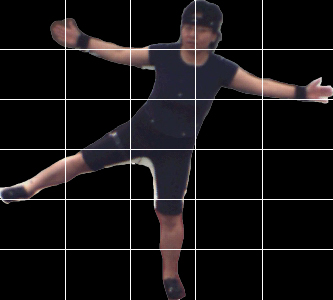
\includegraphics[height=5.5cm]{broad}}\hspace{.5cm}
  \subcaptionbox{较窄图片}{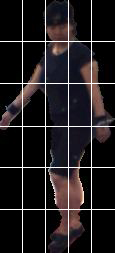
\includegraphics[height=5.5cm]{thin}}
  \caption{图片比例影响示意}\label{fig:broadthin}
\end{figure}

\begin{figure}[htbp]
  \centering
  \subcaptionbox{}{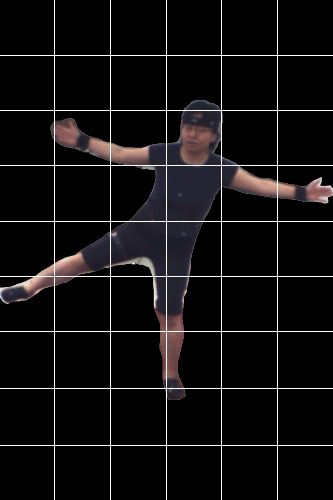
\includegraphics[height=5.5cm]{broad1}}\hspace{.5cm}
  \subcaptionbox{}{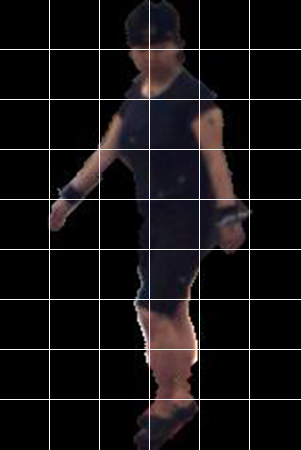
\includegraphics[height=5.5cm]{thin1}}
  \caption{图片固定比例示意}\label{fig:broadthin2}
\end{figure}

每个像素点根据周围像素信息都可以算得一个梯度信息,包括梯度的方向和大小。计算直方图指的是对于每一个元胞,对梯度的方向做直方图,方向范围是$0^\circ\thicksim180^\circ$,将直方图分为9块,每块含$20^\circ$,对在该角度范围的梯度的大小求和作为直方图中这一块的值。每个元胞的直方图统计可以用图\ref{fig:local_hoG}来表示,每一个方向用该方向上的矩形表示,颜色越亮表示梯度越大。最后做L1规范化,得到最终的HOG特征向量。

\begin{figure}[htbp]
  \centering
  \subcaptionbox{完整原图}{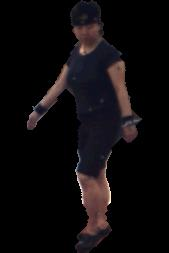
\includegraphics[height=5.5cm]{C1}}\hspace{.5cm}
  \subcaptionbox{右手腕局部}{
\includegraphics[width=0.15\textwidth]{local_org}}\hspace{.5cm}
  \subcaptionbox{单个区域直方图\label{fig:local_hoG}}{
\includegraphics[width=0.15\textwidth]{local_HoG}}
  \caption{HOG特征子区域直方图表示}
\end{figure}

\begin{figure}[htbp]
  \centering
  \subcaptionbox{C1}{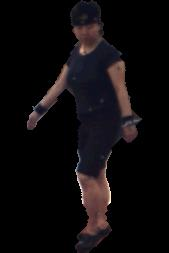
\includegraphics[width=0.2\textwidth]{C1}}\hspace{.5cm}
  \subcaptionbox{C2}{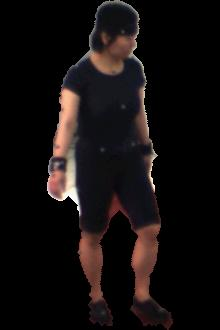
\includegraphics[width=0.2\textwidth]{C2}}\hspace{.5cm}
  \subcaptionbox{C3}{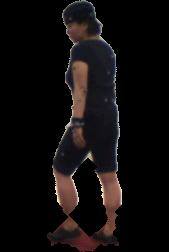
\includegraphics[width=0.2\textwidth]{C3}}\\
  \subcaptionbox{HOG1}{\includegraphics[width=0.2\textwidth]{HOG1}}\hspace{.5cm}
  \subcaptionbox{HOG2}{\includegraphics[width=0.2\textwidth]{HOG2}}\hspace{.5cm}
  \subcaptionbox{HOG3}{\includegraphics[width=0.2\textwidth]{HOG3}}
  \caption{HOG特征}
\end{figure}

\section{皮肤特征}
由于人的皮肤是一个不变的特征,而且胳膊、头的位置对于姿态估计有重要作用,因此充分利用皮肤特征是十分必要的。对于姿态估计,我们只关心胳膊、头的位置,因此本文用位置、面积信息来描述皮肤特征。首先,需要判断每个像素属于皮肤的概率,为了简化问题,本文假定皮肤颜色在YCbCr颜色空间服从高斯分布,均值和方差均为手工给出。由于人们往往是穿着长裤,因此只能检测到头和左右臂这三个部分,而在穿长袖衣服时则只能检测到头和左右手。因此本文只选取概率最大的三个区域\footnote{只考虑ROI中的上半部分。有时候会小于三个区域,因为手和头部相连。},分别认为是头、左臂和右臂。按面积由大到小排序,每一个区域用$\mathbf{r}=(x,y,s)$表示,$(x,y)$为区域的重心坐标,$s$为区域面积。检测结果见图\ref{fig:skin}。
\begin{figure}[H]
  \centering
  \subcaptionbox{原图}{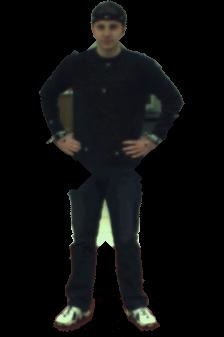
\includegraphics[width=0.3\textwidth]{skin}}\hspace{1cm}
  \subcaptionbox{皮肤检测}{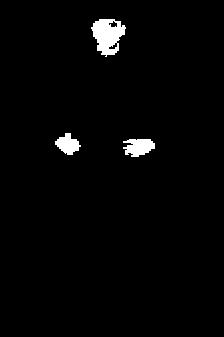
\includegraphics[width=0.3\textwidth]{skinbw}}
  \caption{皮肤检测}\label{fig:skin}
\end{figure}

\section{特征表示}
\label{sec:feature}
HOG特征有$6\times 9=36$个元胞,每个子区域有9维直方图,因此共计$36\times 9=486$维。皮肤特征有3个区域,每个区域$(x,y,s)$三维信息,共计$3\times 3=9$维。两种特征相连共计$486+9=495$维。如果用到三个视角图片,则会有$495\times 3=1485$维。



\chapter{基于双高斯过程的姿态估计算法}

\section{概述}
由第\ref{sec:feature}节和第\ref{sec:skeleton}节可知,本文研究问题的输入输出已经刻画成两个一维向量,记输入向量(特征向量)为$\mathbf{R}$,,输出向量(骨架向量)为$\mathbf{X}$,则$\mathbf{X}=\textrm{F}(\mathbf{R})$,可以归结为一个多输出多元回归问题。显然,输出向量的每个元素之间是有关联的,用若干简单的回归方法(如线性回归、SVM等方法)独立预测各元素是不合理的。此外,我们知道相似的特征应该表示相似的人体骨架,因此,自然想到了 KNN(\emph{k} nearest neighbor regression)算法,但该算法效果并不理想,因此本文采用了一种能更好描述向量之间相关性的算法\pozhehao 双高斯过程回归(Twin Gaussian Process Regression,以下简称TGP)。在介绍该算法前,首先有必要介绍其前身和基础\pozhehao 高斯过程回归(Gaussian Process Regression,以下简称GPR)。

\section{高斯过程回归}
高斯过程回归是基于贝叶斯理论和统计学习理论发展起来的一种机器学习方法, 对于高维数、小样本和非线性等复杂回归问题行之有效。
记输入向量为$\mathbf{R}=(\mathbf{r}_1,\mathbf{r}_2,...,\mathbf{r}_N)$,$dim(\mathbf{r}_i)=W$,对应的输出向量为$\mathbf{X}=(\mathbf{x}_1,\mathbf{x}_2,...,\mathbf{x}_N)$,$dim(\mathbf{x}_i)=D$,N为样例的个数。简单来说,GPR就是假定输入向量的协方差满足高斯分布。先定义$f(\mathbf{r})$ 是输入$\mathbf{r}$的一个函数,用公式\ref{eqn:GPRcov}表示输入向量的协方差,协方差函数可以有多种取法,公式\ref{eqn:GPRguassian}即为一种取法。
  \begin{equation}
  \textmd{cov}\left(f(\mathbf{r}_i),f(\mathbf{r}_j)\right) = K_R\left(\mathbf{r}_i,\mathbf{r}_j\right)\label{eqn:GPRcov}
  \end{equation}
  \begin{equation}
    K_R\left(\mathbf{r}_i,\mathbf{r}_j\right)= \textmd{exp}\left(-\gamma_r||\mathbf{r}_i-\mathbf{r}_j||^2\right)+\lambda_r\delta_{ij}\label{eqn:GPRguassian}
  \end{equation}
其中$\lambda_r$用来描述噪声,
\begin{equation}
  \delta_{ij}=\begin{cases}1,\hspace{1cm}i=j \\ 0,\hspace{1cm}i\neq j  \end{cases}
\end{equation}
又因为$\mathbf{X}=\textrm{F}(\mathbf{R})$,所以有公式\ref{eqn:GPRguassian2}
\begin{equation}\label{eqn:GPRguassian2}
  \begin{bmatrix} {(\mathbf{X}^{(d)})}^\top \\ \mathbf{x}^{(d)} \end{bmatrix}
  \sim \mathcal{N}_R
  \begin{pmatrix}
    \mathbf{0},& \begin{bmatrix} \mathbf{K}_R & \mathbf{K}_R^r \\ {\left(\mathbf{K}_R^r\right)}^\top & K_R(\mathbf{r},\mathbf{r}) \end{bmatrix}
  \end{pmatrix}
\end{equation}

其中$\mathbf{X}^{(d)}$是$\mathbf{X}$的第\emph{d}列,$\mathbf{x}^{(d)}$是$\mathbf{x}$的第\emph{d}个元素;$\mathbf{K}_R$是$N\times N$矩阵,$(\mathbf{K}_R)_{ij}=K_R(\mathbf{r}_i,\mathbf{r}_j)$;$\mathbf{K}_R^r$是$N\times 1$的向量,$\left(\mathbf{K}_R^r\right)_{ij}=K_R(\mathbf{r}_i,\mathbf{r})$,用来描述输入向量的相关性;$K_R(\mathbf{r},\mathbf{r})$是$\mathbf{r}$自身的协方差。

用$\mathbf{X}^{(d)}$表示观测数据,$\mathbf{x}^{(d)}$表示预测数据,因为二者联合分布符合高斯分布,因此后验概率$p(\mathbf{x}^{(d)}|(\mathbf{X}^{(d)})^\top)$ 也满足高斯分布,均值和方差分别见公式\ref{eqn:GPRmean}、\ref{eqn:GPRvar},即可用均值表示输入$\mathbf{r}$的预测结果。
\begin{equation}\label{eqn:GPRmean}
  \textmd{mean}\left(\mathbf{x}^{(d)}\right) = \mathbf{X}^{(d)} \mathbf{K}_R^{-1} \mathbf{K}_R^r
\end{equation}
\begin{equation}\label{eqn:GPRvar}
\sigma^2\left(\mathbf{x}^{(d)}\right) = K_R\left(\mathbf{r},\mathbf{r}\right) - {\left(\mathbf{K}_R^r\right)}^\top \mathbf{K}_R^{-1} \mathbf{K}_R^r\
\end{equation}

以上阐述了如何利用GPR进行预测,关于GPR的参数如何学习计算,可以采用共轭梯度法、牛顿法等优化方法求得参数的最优解,本文不再详述。

由于GPR只关心单个输出的预测,没有考虑每个输出之间的关系,而且对于从二维平面恢复三维姿态这样一个多解问题GPR显得无能为力,因此本文采用了双高斯过程回归,将在\ref{sec:TGP} 节介绍。

\section{双高斯过程回归}
\label{sec:TGP}
\subsection{概述}
为了考虑各输出变量之间的相关性,借鉴GPR的思路,我们假定输出变量之间也符合关于输出的高斯分布:
\begin{equation}
  \begin{bmatrix} {\left(\mathbf{X}^{(d)}\right)}^\top \\ \mathbf{x}^{(d)} \end{bmatrix} \sim \mathcal{N}_X\left(\mathbf{0},\mathbf{K}_{\mathbf{X}\bigcup \mathbf{x}}\right)
\end{equation}

其中相关性矩阵为:
\begin{equation}
  \mathbf{K}_{\mathbf{X}\bigcup \mathbf{x}} = \begin{bmatrix} {\left(\mathbf{X}^{(d)}\right)}^\top \mathbf{X}^{(d)} & {\left(\mathbf{X}^{(d)}\right)}^\top \mathbf{x}^{(d)}
\\ \mathbf{X}^{(d)} \mathbf{x}^{(d)} & \mathbf{x}^{(d)} \mathbf{x}^{(d)}
 \end{bmatrix}
\end{equation}

于是$\begin{bmatrix} {\left(\mathbf{X}^{(d)}\right)}^\top \\ \mathbf{x}^{(d)} \end{bmatrix}$服从$\mathcal{N}_X$和$\mathcal{N}_R$两个正态分布。我们希望这两个分布尽量一致,$\mathcal{N}_X$ 的参数是需要估计的,通过优化调整$\mathbf{x}^{(d)}$使两个分布尽量接近。

\subsection{KL散度}
为了刻画相同事件空间里的两个概率分布的相似度,在此引入KL散度(Kullback-Leibler Divergence),其物理意义是:在相同事件空间里,概率分布$P(x)$ 的事件空间,若用概率分布$Q(x)$ 编码时,平均每个基本事件(符号)编码长度增加了多少比特\footnote{url:\url{http://en.wikipedia.org/wiki/Kullback-Leibler_divergence}}。 计算公式为:
\begin{equation}
  D(P||Q)=\sum P(x)\log \frac{P(x)}{Q(x)}
\end{equation}

具体在这里$\mathcal{N}_X$和$\mathcal{N}_R$的KL散度可表示为:
\begin{align}
 D_{KL}(N_X||N_R) &= -\frac{N}{2}-\frac{1}{2}\log|\mathbf{K}_{\mathbf{X}\bigcup \mathbf{x}}| \notag\\
                  &+ \frac{1}{2}\textmd{Tr} \begin{Bmatrix} \mathbf{K}_{\mathbf{X}\bigcup \mathbf{x}} \begin{bmatrix} \mathbf{K}_R & \mathbf{K}_R^r \notag\\ {\left(\mathbf{K}_R^r\right)}^\top & K_R(\mathbf{r},\mathbf{r}) \end{bmatrix} ^{-1} \end{Bmatrix}\\
                  &+ \frac{1}{2}\log \begin{vmatrix}\begin{bmatrix} \mathbf{K}_R & \mathbf{K}_R^r \\ {\left(\mathbf{K}_R^r\right)}^\top & K_R(\mathbf{r},\mathbf{r}) \end{bmatrix}\end{vmatrix}\label{eqn:KLorg}
\end{align}

于是预测三维姿态$\mathbf{x}$转化成一个优化问题:
\begin{equation}
  \mathbf{x}^\ast  = \underset{\mathbf{x}^{(d)}}{\textmd{argmin}} \left[L\left(\mathbf{x}^{(d)}\right)\equiv D_{KL}(N_X||N_R)\right]
\end{equation}

其中Tr表示求矩阵的迹。
\subsection{求解优化问题}
通过去掉公式\ref{eqn:KLorg}中和$\mathbf{x}$的无关项,加以简化可以得到式\ref{eqn:KL1}
\begin{align}
 L\left(\mathbf{x}^{(d)}\right) &= \mathbf{x}^{(d)}\mathbf{x}^{(d)}-2\mathbf{x}^{(d)} \mathbf{X}^{(d)} \mathbf{K}_R^{-1} \mathbf{K}_R^r \notag\\
               &- \left[K_R(\mathbf{r},\mathbf{r}) - \left(\mathbf{K}_R^r\right)^\top \mathbf{K}_R^{-1} \mathbf{K}_R^r\right] \notag\\
               &\times \log\left\{\mathbf{x}^{(d)}\mathbf{x}^{(d)} - \mathbf{x}^{(d)}\mathbf{X}^{(d)} \left[{\left(\mathbf{X}^{(d)}\right)}^\top \mathbf{X}^{(d)}\right]^{-1} {\left(\mathbf{X}^{(d)}\right)}^\top \mathbf{X}^{(d)} \right\}\label{eqn:KL1}
 \end{align}

 如果预测三维姿态变量各维之间是独立的,那么可以写成公式\ref{eqn:KL2}
 \begin{align}
 L(\mathbf{x}) &= \mathbf{x}^\top\mathbf{x}-2\mathbf{x}^\top \mathbf{X} \mathbf{K}_R^{-1} \mathbf{K}_R^r \notag\\
               &- \left[K_R(\mathbf{r},\mathbf{r}) - \left(\mathbf{K}_R^r\right)^\top \mathbf{K}_R^{-1} \mathbf{K}_R^r\right] \notag\\
               &\times \log\left[\mathbf{x}^\top\mathbf{x} - \mathbf{x}^\top\mathbf{X}
               \left({\mathbf{X}}^\top \mathbf{X}\right)^{-1} {\mathbf{X}}^\top \mathbf{X}\right]\label{eqn:KL2}
 \end{align}

然而显然变量各维之间是不独立的,因此同对待输入变量一样,我们为输出变量各维之间也定义相关函数:
\begin{equation}
  \textmd{cov}\left(f(\mathbf{x}_i),f(\mathbf{x}_j)\right) = K_R\left(\mathbf{x}_i,\mathbf{x}_j\right)\label{eqn:TGPcov}
\end{equation}

同样相关函数也可以选择和公式\ref{eqn:GPRguassian}类似的高斯函数。于是我们把输出变量的相关矩阵表示为式\ref{eqn:TGPcov2}
\begin{equation}
    \mathbf{K}_{\mathbf{X}\bigcup \mathbf{x}} = \begin{bmatrix} \mathbf{K}_X & \mathbf{K}_X^x \\ {\left(\mathbf{K}_X^x\right)}^\top & K_X\left(\mathbf{x},\mathbf{x}\right) \end{bmatrix}\label{eqn:TGPcov2}
\end{equation}

于是最终优化问题变为式\ref{eqn:TPGopt}
\begin{align}
 L(\textbf{x}) &= K_X\left(\textbf{x},\textbf{x}\right)-2\left(\textbf{K}_X^x\right)^\top \textbf{K}_R^{-1} \textbf{K}_R^r \notag\\
               &- \left[K_R(\textbf{r},\textbf{r}) - \left(\textbf{K}_R^r\right)^\top \textbf{K}_R^{-1} \textbf{K}_R^r\right] \log\left[K_X(\textbf{x},\textbf{x}) - \left(\textbf{K}_X^x\right)^\top \textbf{K}_X^{-1} \textbf{K}_X^x\right] \label{eqn:TPGopt}
 \end{align}

通过求取梯度,令梯度为0,即可求得最优解。

\section{TGPKNN}

由于TGP方法需要求$N\times N$矩阵的逆,当$N$很大时复杂度会很高,因此需要做一定的近似来降低复杂度,在这里考虑用KNN($k$ nearest neighbors)方法先在$N$个数据中选择$k$个和待预测数据最接近的,然后再用TGP来实现。



\chapter{结果分析与比较}

\section{运行环境}


\chapter{总结与展望}
\section{总结}
本文实现了一种可以估计人体三维姿态的算法,在大量数据上进行了测试。测试结果并不理想,和原文有较大差距。在实验的过程中,我发现了一些问题,比如即便ground-truth告诉我们当前帧的运动捕捉到的姿态是有效的,实际可能是错误的,可以参照图\ref{fig:wrong}。
\begin{figure}[H]
  \centering
  \subcaptionbox{原图}{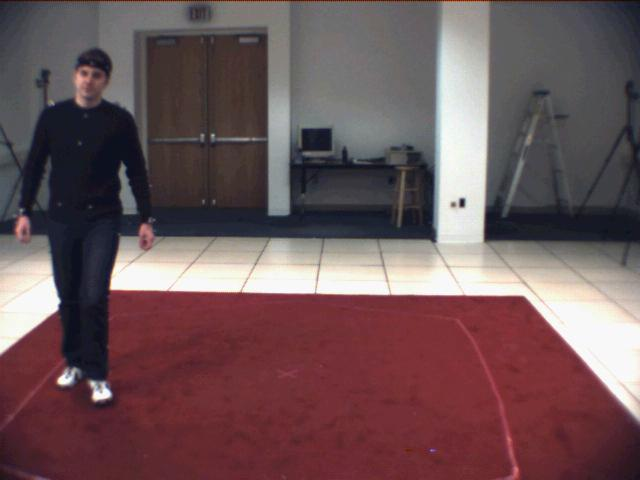
\includegraphics[height=5.5cm]{wrongimage}}
  \subcaptionbox{错误骨架}{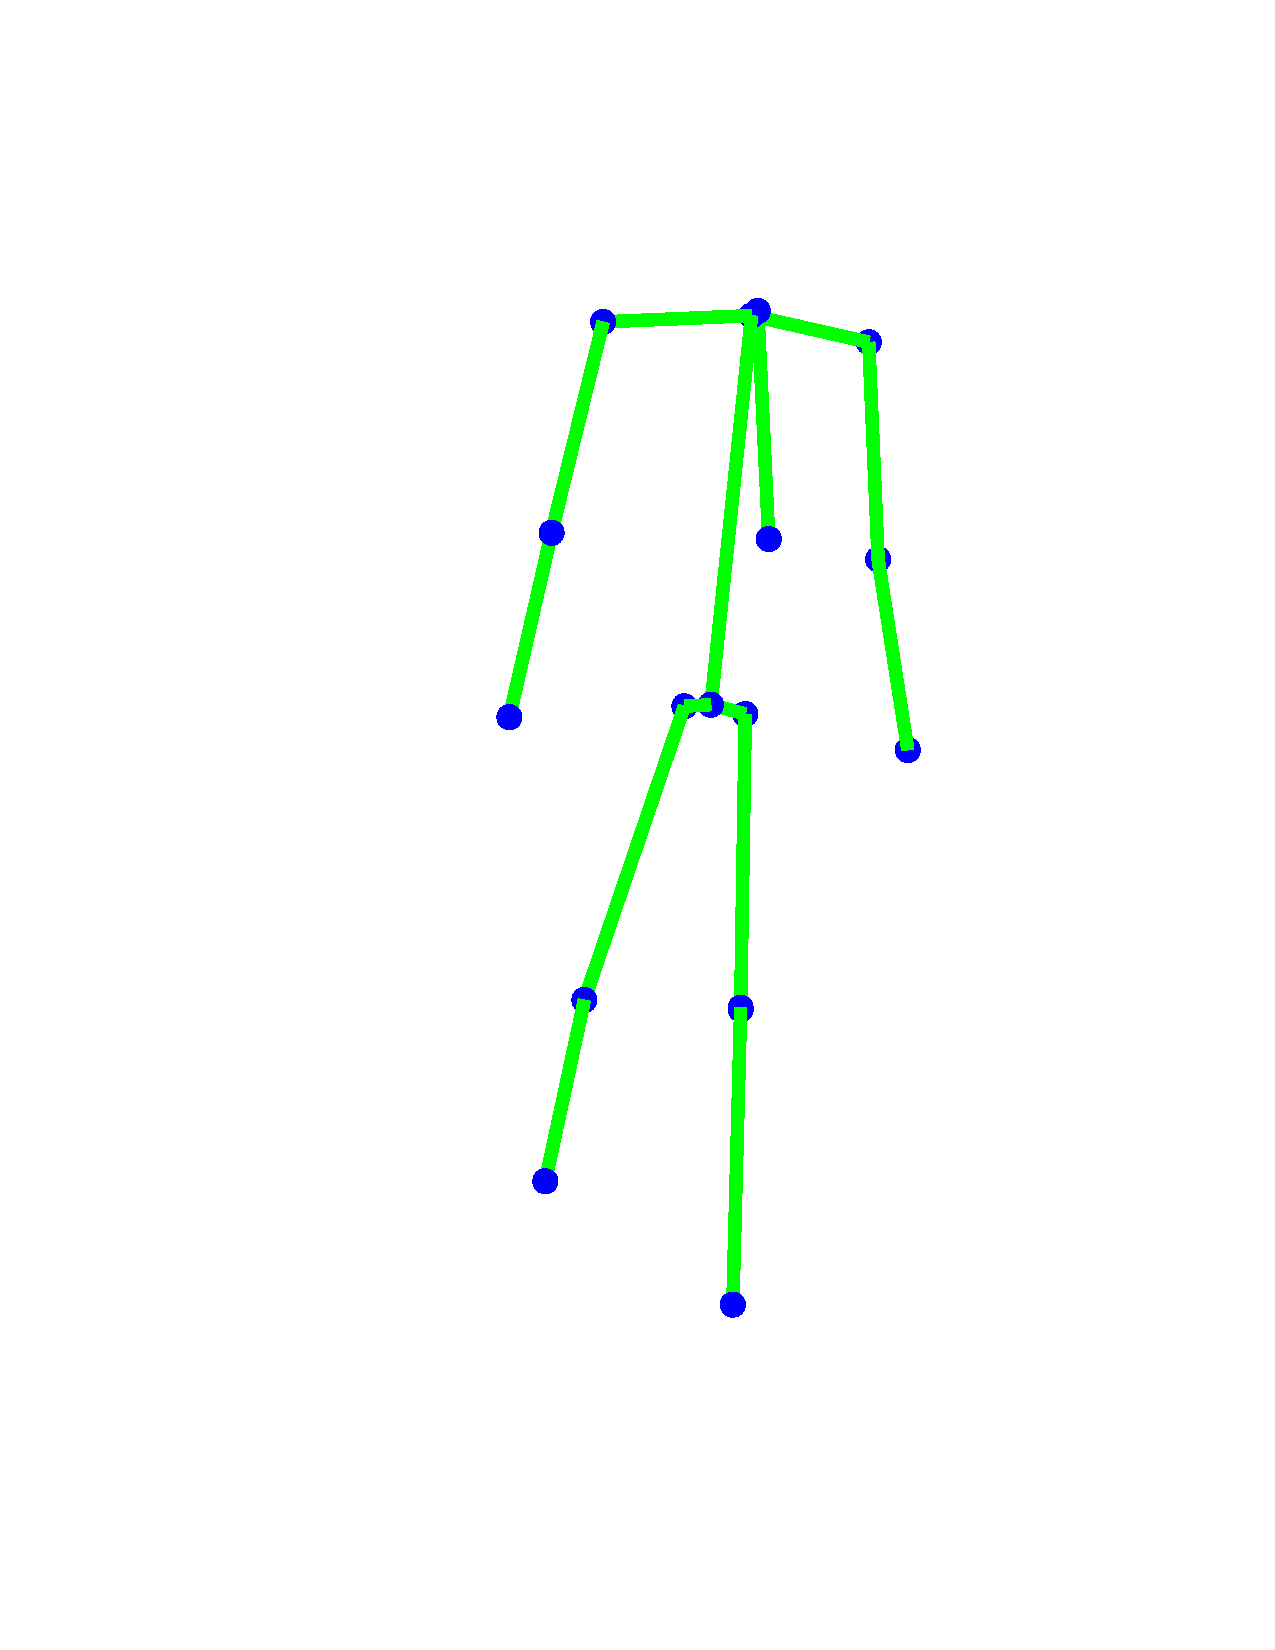
\includegraphics[height=5.5cm]{wrong}}
  \caption{错误的ground-truth}\label{fig:wrong}
\end{figure}

本文采用了不同的特征得到了较差的结果,说明了预测结果和特征关系极大,由于这次的实验十分耗时,我没能用更多的时间去选择合适的特征,我非常遗憾。在接下来的工作中,我希望能提出一种更有效的特征来解决这个问题。HOG特征本身是有结构的,可以先把每个元胞作为一维特征进行训练分类,再根据元胞的梯度信息进行回归,将有可能降低复杂度并提高准确率。但是只去选择更合适的特征意义并不大,综合一些文献~\cite{ramanan2007learning}~\cite{yang2011articulated}的思路,我认为在解决人体姿态估计问题中需要分层处理,即先识别各个肢体的位置和姿态,然后再全局优化。用本文中所述将所有信息一起训练是冗余且低效的,即使用了多达10000帧的数据,并且动作简单到只有几类,效果仍然不是很好。只有好的特征配合高效的算法才能实现更好的预测结果。

\section{收获与体会}
首先,我认为选题是非常重要的环节。在毕业设计初期,我一直在做很多尝试,调查了很多方向,也阅读了相当多的文献,但都没有找到合适的方向下手。当考虑做多人体三维建模时发现难度很大,于是不断缩小目标,最后落脚到单人体三维姿态估计,即便如此,经过调查我发现这是一个由来已久的难题,于是只好摸索着前进。前期调研花掉了较多的时间,导致后期做实验的时间被大大缩短,也导致了结果的不理想。

其次,我体会到了做图像处理实验的难处。第一,数据库很重要,巧妇难为无米之炊,也正如文献~\cite{gkiox2013ariarticulated}所说那样:\\
\begin{center}
\shadowbox{
\begin{minipage}{8cm}
\thispagestyle{plain}
We give the last word to Sherlock Holmes:\\
“Data! Data! Data!” he cried impatiently. “I can't make bricks without clay.”\\
\emph{The Adventure of the Copper Beeches}
\end{minipage}}
\end{center}
没有数据就没办法实验,好在本文可以利用HumanEva数据库,在此十分感谢布朗大学。第二点难处是时间,做实验非常漫长,需要很好的耐心,不能轻易放弃。在我没有结果的时候,我的朋友给了我鼓励和帮助,让我坚持了下去,我很感激他们。

当然,我收获了很多知识,不仅仅是人体姿态识别这个领域我了解了最流行最有效的方法,我还在前期调研中探索了很多其他领域,比如图片拼接、3D视频质量评价、去模糊、三维重建、霍夫树等。收获的也不止是知识,还有学习的方法,熟悉了如何调研、查阅文献,怎么去网上找到可以利用的代码和数据库等等。 

%%% 其它部分
\backmatter

% 本科生要这几个索引,研究生不要。选择性留下。
\makeatletter
\ifthu@bachelor
  % 插图索引
  \listoffigures
  % 表格索引
  \listoftables
  % 公式索引
  \listofequations
\fi
\makeatother

\newif\ifpdf
\pdffalse
\ifpdf
\else
    % 参考文献
    \bibliographystyle{thubib}
    \bibliography{ref/refs}
\fi

% 致谢
%%% Local Variables:
%%% mode: latex
%%% TeX-master: "../main"
%%% End:

\begin{ack}
  感谢导师戴琼海教授、刘烨斌老师对本人的热情指导,他们帮助我迈出了科研的第一步,做科研的方法将终身受益。
  
  承蒙王雁刚师兄的指导和帮助,我坚定了研究方向,梳理了研究思路,在做不下去的时候,王雁刚师兄一次次给予了我前进的方向和成功的信心。
  
  感谢和我一起讨论问题、交流毕业论文心得的吴蒙蒙、刘金林、胡雪梅等同学,是你们,让毕业设计有了更多的欢声笑语。
  
  最后感谢柯家琪、张洋师兄对我撰写论文给予的帮助,感谢 \thuthesis,它的存在让我的论文写作轻松自在了许多,让我的论文格式规整漂亮了
  许多。
  
\end{ack}


% 附录

\ifpdf
    \begin{appendix}
    %%%% Local Variables:
%%% mode: latex
%%% TeX-master: "../main"
%%% End:

\chapter{外文资料翻译}
\pagestyle{empty}
%\includepdfset{pagecommand={\thispagestyle{thu@plain}}}
%\includepdf[pages=1-8]{data/FFDB.pdf} %标题
\begin{center}
\sanhao{一种用于视频中表情生成的数据驱动方法}\\
\vspace{10pt}
\wuhao
李凯$^{1,2}$ \text{~~~~} 徐枫$^{1}$ \text{~~~~}王珏$^{3}$ \text{~~~~}戴琼海$^{1}$ \text{~~~~}刘烨斌$^{1}$\\
$^{1}$清华大学自动化系\\
$^{2}$清华大学深圳研究院\text{~~~}
$^{3}$Adobe 系统\\
\end{center}

%摘要
\CJKfamily{hei}\textbf{摘要:}
\CJKfamily{kai}
本文提出了一种方法来用一个人的面部表情视频对目标人脸合成真实的面部动画。不用于以往的面部动画方法,我们的系统利用了现有的目标人物的面部表情数据库,并最终通过从数据库中获取含有与输入相似的表情的帧来生成最终视频。为此我们开发了一种表情相似度度量来准确地测量两个视频帧的表情差异。为了加强时间相干性,我们的系统从相似度度量决定的候选帧中,利用最短路径算法来选择最优的图片。最后,我们的系统采用一种表情映射的方法来进一步减小输入和检索得到的帧之间的表情差异。实验结果显示我们的系统可以利用所提出的数据驱动方法生成高质量面部动画。
%\noindent
%\CJKfamily{hei}\textbf{关键字:}
%\CJKfamily{kai}
%多角度立体视觉,融合,点云,矩阵恢复,压缩感知。

%正文
\CJKfamily{song}
\section{简介}
性能驱动的面部动画在20世纪80年代就已经走红。它指的问题是:将面部表情从一个人映射到另一个,目标是使渲染的目标面部动画和原表情相比真实且一致。

尽管在过去几十年内已经取得了巨大进步,但这个问题依然未解决。之前的方法主要集中于表情的真实度,也就是说,使目标面部的渲染表情主观上接近输入面部的表情。另一方面,逼真的渲染很大程度上被忽视,先前的方法通常使用3D面部模型作为目标头像。目前尚不清楚在给出一个人的表情后,怎样为一个真实人物的面部渲染逼真的动画。此外,许多以前的方法严重依赖诸如在源面部上标记\cite{feature_based, eri},或精细的人机交互做跟踪\cite{performance_driven, drawing}等额外信息。这些方法的应用范围和效率因此比较有限。

在本文中,我们旨在开发一种自动化系统将一个脸部视频的表情转化到另一个人上,从而产生目标人物的自然表情的视频。受到最近在封闭人脸实现~\cite{deng}和人体运动动画~\cite{xufeng}上的数据驱动方法的启发,我们的系统基于现有的目标人物的表情数据库来实现目标。由于数据库提供了目标人脸在不同表情下的自然视频帧,我们可以利用这些做参考来渲染和输入表情匹配的视频。然而,这个任务并不简单,有如下挑战:
\begin{enumerate}[1.]
  \item 怎样测量两个不同人物视频帧的表情相似度;
  \item 怎样高效地搜索数据库以确保生成的视频不仅接近输入表情,也具有时间相干性;
  \item 由于数据库大小有限,不能覆盖所有输入的表情,怎样进一步调整目标视频帧的表情来提高表情准确性。
\end{enumerate}
我们的系统采用一套技术来解决这些挑战。具体来说,我们提出一个新颖的测量视频中不同人物表情的相似度。为了在时间相干性和表情匹配精度上平衡,我们先从数据库找到K近邻作为每个输入帧的候选,用优化方法来求得最优输出序列。最后,考虑到每个输入和检索帧的细微表情差异,我们提出一种表情转移方法,用这个结果来进一步细化获得的帧的表情。实验结果显示我们的系统能合成时间上连贯且与输入匹配的逼真的面部表情动画。
\section{相关工作}
这项工作与以前在面部表情匹配、面部表情重定向(映射)、视频到视频合成方面研究工作相关。
\subsection{面部表情匹配}
我们的要求是找到最相似的苗青,而不是把面部运动分类到具体、事先定义的类别。在表情识别社区中使用的特征,比如Gabor小波~\cite{Gabor}, LBP~\cite{lbp}和FACS~\cite{facs},或许能提供一种替代方法。然而,他们经常没能考虑身份的差异。比如,一个有胡子的笑脸与没有胡子的笑脸,就LBP特征而言是不同的。只有拥有足够的有胡子和没胡子的训练样本,分类器才能辨别两个笑脸是一样的。此外,这些度量也许不能推断出一个连续的实值距离测量,这意味着他们经常不足以精确地捕捉细微的表情差异。比如CERT~\cite{CERT},仅仅能较好识别峰值表情的活动单元。还不清楚它分辨细微的AU运动能有多好。相反,这两个主要问题在我们提出的表情相似度测量中不存在。

\subsection{3D基于模型的面部表情重定位}
在表情建模和重定位方面已有大量工作。在基于PCA的模型中,比如AAM~\cite{AAM}\\ /CLM~\cite{Saragih},3D形变模型~\cite{morphable},多线性模型~\cite{multilinear,replacement},和变形模型~\cite{face_off},通用基础通过保留主成分从大训练数据中学习来。他们以丢失精细的细节为代价努力换取鲁棒地跟踪所有表情。然而在我们的精炼方法中,在两个相似表情的图片中光流可以更好地捕捉细节表情的不同,从而获得更精确地重定位结果。有特殊特征的形状融合模型为实时动画而建立~\cite{realtime_kinect}。然而,形状融合变形器的数量是模型覆盖度和很总适应性之间的矛盾。其他系统~\cite{photographs,cloning,reanimating} 努力建立纹理逼真的3D面部模型。然而,获得完全纹理p的3D模型并不容易。

\subsection{基于图片的表情映射}
一些人脸合成系统直接在2D图片上操作来实现表情转移。Williams的系统~\cite{performance_driven}从源和目标图片提取面部特征,用特征差异引导扭曲。Liu等人~\cite{eri} 提出 Expression Ratio Image (ERI)通过捕捉光照变化来加强表情映射。Zhang\emph{ et al.}~\cite{geometry_driven}用几何元通过融合样例脸部图片来计算每个图片子区域的纹理。然而,这些方法通常不能处理两幅图片间大的拓扑变化。我们的方法通过从拥有和输入相似的表情的数据库中获得目标脸部克服了这个局限。此外,这些方法通常是劳动密集型的。

\subsection{视频到视频的合成}
我们的工作涉及到之前视频到视频合成系统。和我们的目标相似,Kemelmacher-Shlizerman等人~\cite{eccv10}利用数据库,在一个人联视频驱动下合成一个目标人物的面部视频。然而,他们的系统主要着眼于测量面部表情的相似度。最终视频只是简单地由独立的最相似的图片连接合成,这可能时间上不一致。视频面部替代系统~\cite{replacement} 在保证时空一致性的基础上用源视频的面部代替目标视频中的人脸。然而,它假设输入和目标视频之间粗糙的语义对应和大致相近。

\section{系统概览}
\renewcommand{\figurename}{图}
\begin{figure}[htbp]
\centering
    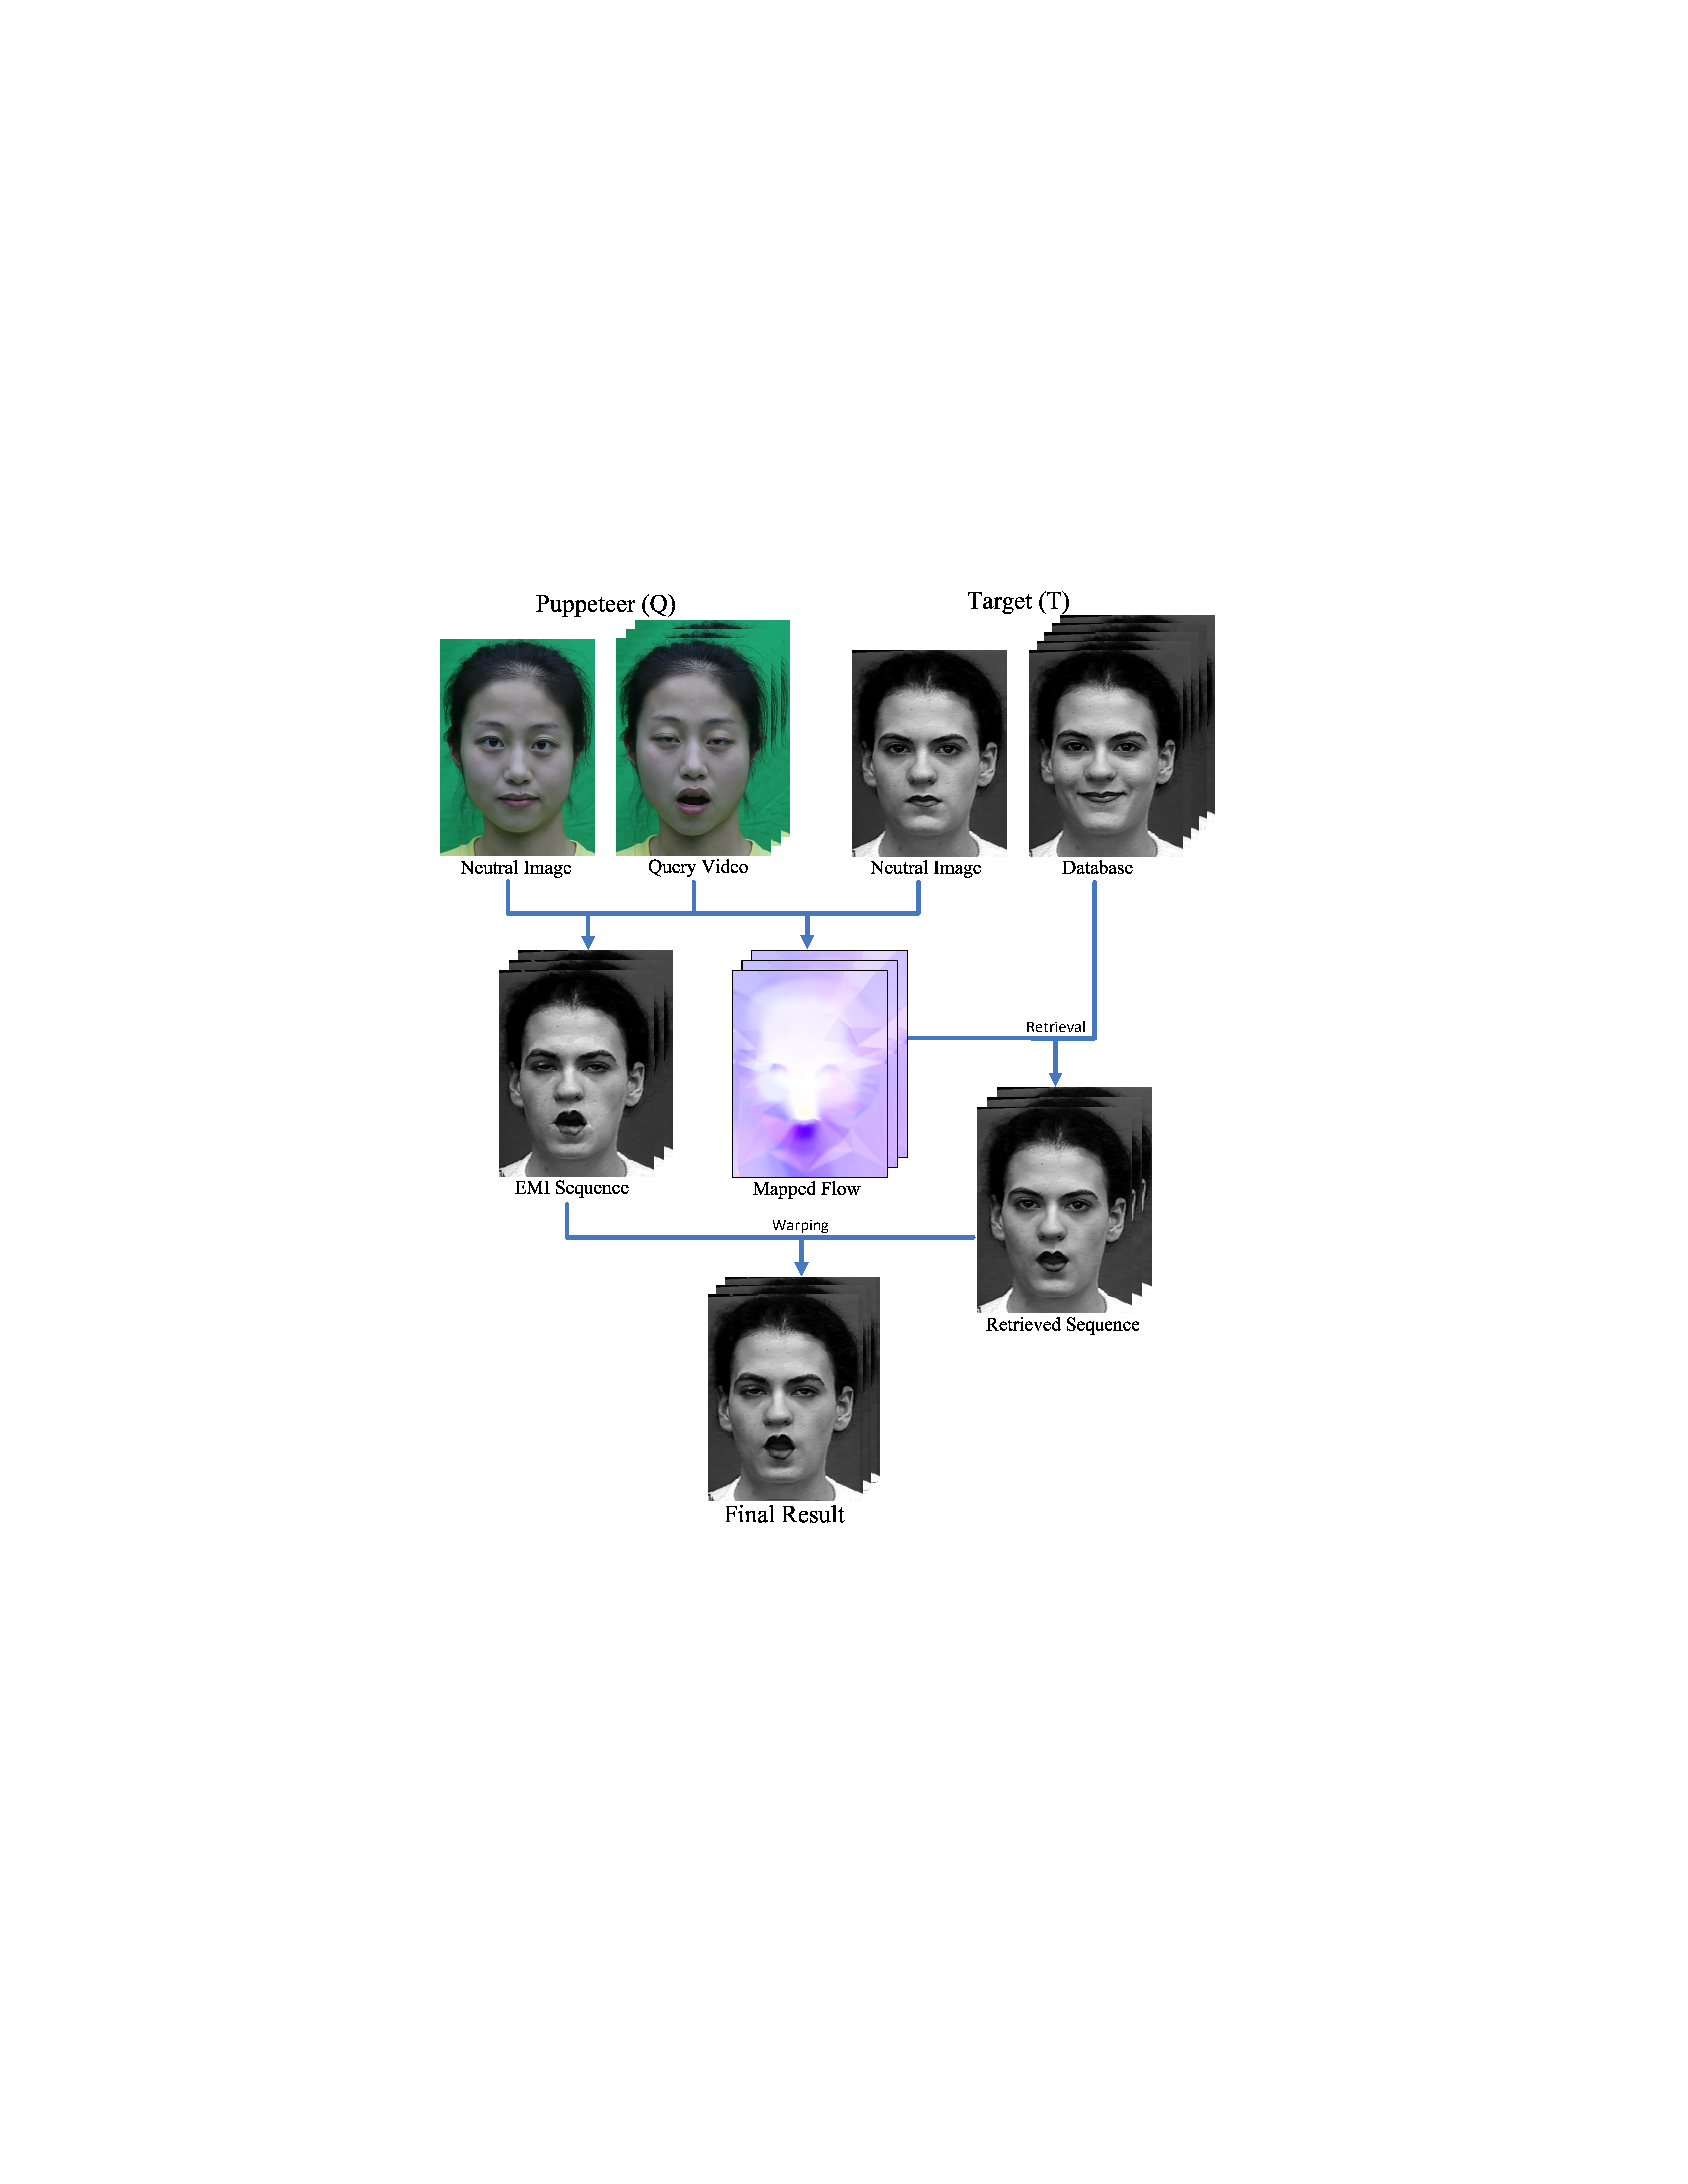
\includegraphics[width=0.95\textwidth]{data/img/overview.pdf}
    \caption{系统概览. 首先将每个查询帧和它的中性面部之间的光溜映射到目标人,用来从数据库中检索。同时,目标人的中性图像被扭曲以生成含有查询表情的EMI序列。最后,检索序列用EMI 精炼,来生成最终结果。}
    \label{fig:overview}
\end{figure}
图~\ref{fig:overview}展示了我们系统的概况。要为目标人生成逼真的表情,我们首先捕捉一段这个人展示基本表情的视频,比如生气、恐惧、惊奇、伤心、高兴、厌恶。有了另一个我们叫做人偶师(puppeteer)的人的面部表情,我们的方法尝试利用目标人的数据合成同样的表情。

具体而言,对于每个输入帧,我们使用第~\ref{sec:metric}章描述的基于光流相似度度量方法查询数据库获得$k$个与输入帧有最相近表情的目标人的视频帧。正如在第~\ref{sec:retrieval} 章描述的那样,我们把这个任务认为是和最短路问题一样找最优连续帧,而不是像Kemelmacher-Shlizerman等人~\cite{eccv10} 直接用最相似的帧生成一个匹配序列。获得的序列包含和人偶师相似且时间一致的表情。

然而,由于数据库大小有限,为每个输入帧找到一个完美的表情匹配几乎是不可能的,更何况,一些表情的人偶师具有独特的特点。为了考虑再输入和检索帧之间细微的表情差异,我们用一个表情映射技术来生成另一个候选面部,我们称之为EMI图像,如第~\ref{sec:emi}章描述那样。EMI图片通常有比检索帧有更精确的面部表情,但她的面部外观可能有重大瑕疵。在最后一步,我们把EMI图片和检索帧结合起来从而生成有精确表情和逼真外观的最终输出帧,如第~\ref{sec:emi}章所述。
\section{算法}
\subsection{表情相似度度量}\label{sec:metric}
给出人偶师的面部图片$Q_e$, 我们的系统试图从目标人的数据库中找到对应面部图片$T_e$,这幅图片有和$Q_e$最接近的面部表情. 为此我们需要能准确测量$Q_e$ 和 $T_e$之间表情差异的面部相似度度量, 同时忽视两幅图片的外表差异。

为了找到这样一个度量,我们的系统使用人偶师和目标人的中性面,分别记作$Q_n$ 和 $T_n$。当我们建立数据库的时候 $T_n$ 只需要标识一次,我们假设 $Q_n$ 在输入视频中由用户标记。为了说明人偶师的面部如何从 $Q_n$ 到 $Q_e$变化,我们能计算两幅图片中的光流场~\cite{celiu}记作 \mbox{\boldmath $F$}$_{Q_n \to Q_e}\in\mathbb{R}^{m \times 2}$, 这里$m$表示$Q_n$中的所有人脸像素。为了从光场中去除全局头部运动,我们用不随表情变化的鼻子区域来估计2D相似度变化,在计算表情差异前先把$Q_e$和$Q_n$对齐。我们也用脸的宽度归一化光流。类似的,$T_n$和$T_e$之间的光流场\mbox{\boldmath $F$}$_{T_n \to T_e}\in\mathbb{R}^{n \times 2}$, 其中$n \neq m$, 也可以计算。然而,由于身份/外观不同我们不能直接对比这两个光场。
\begin{figure}[htbp]
\centering
    \subcaptionbox{面部标记}{
    \label{fig:face_marker}
    \includegraphics[width=0.20\textwidth]{data/img/facemarker.pdf}}
    \hspace{5mm}
    \subcaptionbox{局部区域}{
    \label{fig:face_region}
    \includegraphics[width=0.20\textwidth]{data/img/faceregion.pdf}}
    \caption{中性脸初始化 (a) 绿色是ASM的标记,红色是手工标记
    (b) 眼睛、嘴巴、鼻子区域分别用品红、蓝色、绿色标记。}
    \label{fig:face}
\end{figure}
为了在两个光场之间建立精确的对应,我们首先使用Active Shape Model (ASM)~\cite{asm}只检测在中性面$Q_n$和$T_n$的面部标志物,该方法对于中性表情的正面人脸很有效。然而它无法覆盖我们算法在之后几步中需要的所有面部。因此我们在两个中性面上手工标注标志点,如图~\ref{fig:face_marker}所示。然后我们用Delauney三角网标出$Q_n$ 和 $T_n$ 中的脸部区域,这引出一个只能像素注册函数$g: Q_n \to T_n$。此外,由于两个身份之间的语义对应应该对不同的面部表情具有不变性,可以合理假设$g': Q_e \to T_e$两个表情图片的注册函数近似和$g: Q_n \to T_n$ 相同。有了注册函数,对于一个点$\vec{a}\in Q_n$转移到$\vec{a}' \in Q_e$,它在$T_n$对应的光流向量按如下计算:
\begin{equation}\label{eq:map2}
\Delta \vec{b}=g(\vec{a}')-g(\vec{a}),
\end{equation}
其中$\vec{b}=g(\vec{a})$是$T_n$上$\vec{a}$的对应点。

通过在$Q_n$上的所有面部像素应用这个映射,我们获取了一种映射好的光流场\mbox{\boldmath $F$}$'_{Q_n \to Q_e}$,可以通过与\mbox{\boldmath $F$}$'_{Q_n \to Q_e}$对比测量两个表情有多接近。以往工作指出~\cite{eccv10},表情差异的主要来源是眼睛和嘴巴区域,因此我们只用这些区域的像素来计算表情相似度(参见图~\ref{fig:face_region})。直接的方法是通过绝对的光流差计算$Q_e$ 和 $T_e$之间的表情差异:
\setlength\arraycolsep{1pt}
\begin{eqnarray}\label{eq:dist_mag}
d_e(Q_e, T_e)&=& \alpha_{e}\sum_{i\in\text{eye}}\left\|F'_{Q_n \to Q_e,i} -F_{T_n \to T_e,i}\right\| \nonumber\\
  &&+\alpha_{m}\sum_{i\in\text{mouth}}\left\|F'_{Q_n \to Q_e, i} -F_{T_n \to T_e, i}\right\|,
\end{eqnarray}

这里下标$i$表示光流矩阵\mbox{\boldmath $F$}中第$i$行。$\alpha_{\{e, m\}}$分别是眼睛和嘴巴区域的权重。
\begin{figure}[htbp]
\centering
    \subcaptionbox{}{
    \label{fig:metric_driven}
    \includegraphics[width=0.2\textwidth]{data/img/metric_likai_0380_00103.pdf}}
    \subcaptionbox{}{
    \label{fig:metric_lbp}
    \includegraphics[width=0.2\textwidth]{data/img/metric_lbp_00102.pdf}}
    \subcaptionbox{}{
    \label{fig:metric_mag}
    \includegraphics[width=0.2\textwidth]{data/img/metric_OFmag_00102.pdf}}
    \subcaptionbox{}{
    \label{fig:metric_magori}
    \includegraphics[width=0.2\textwidth]{data/img/metric_OFmagori_00102.pdf}}
    \caption{表情度量对比。 (a) 查询帧。 (b) 由LBP方法得到的最相似表情,它有一个不理想的皱眉。 (c) 由等式~\ref{eq:dist_mag}获得的最相似表情,有一个笑容而不是惊奇。 (d) 由等式~\ref{eq:dist_comb}获得的最相似表情,和查询帧匹配很好}
    \label{fig:metric}
\end{figure}

等式~\ref{eq:dist_mag}中的距离度量在我们大多数实验中都很成功,但我们发现会偶尔产生如图~\ref{fig:metric}所示的错误。这是因为在等式~\ref{eq:dist_mag}中,我们仅考虑了\mbox{\boldmath $F$}$'_{Q_n \to Q_e}-$\mbox{\boldmath $F$}$_{T_n \to T_e}$的光流差异的大小。但光流的方向通常包含更多有关表情的重要信息。比如笑脸通常与嘴角的上翘相关,而哭脸和嘴角下弯相关。这表明在$Q_e$中的表情与$T_e$中的很不一样,如果\mbox{\boldmath $F$}$'_{Q_n \to Q_e}$到\mbox{\boldmath $F$}$_{T_n \to T_e}$的差异方向很不一样,即便差异大小很小。有了这个发现,我们重新设计表情距离度量如下:
\setlength\arraycolsep{1pt}
\begin{eqnarray}
d_b(\vec{u},\vec{v})&=&\beta_m|\vec{u}-\vec{v}|+\beta_o(-\vec{u}\cdot\vec{v}+|\vec{u}||\vec{v}|), \label{eq:d0}\\
d_e(Q_e, T_e)&=&\alpha_{e}\sum_{i\in\text{eye}}d_b(F'_{Q_n \to Q_e,i}, F_{T_n \to T_e,i})\nonumber\\
           &&+\alpha_{m}\sum_{i\in\text{mouth}}d_b(F'_{Q_n \to Q_e, i}, F_{T_n \to T_e, i}),\label{eq:dist_comb}
\end{eqnarray}

这里$\beta_{\{m, o\}}\in[0,1]$分别是大小和方向的权重,且$\beta_m+\beta_o=1$。 当$\beta_o$ 等于零,等式~\ref{eq:dist_comb}简化为等式~\ref{eq:dist_mag}。在等式~\ref{eq:d0} 中的偏移量$|\vec{u}||\vec{v}|$确保方向项非负。注意此距离度量不保证对称性和三角不等式。为使之更有数学味,可以计算反向距离$d_e(T_e,Q_e)$,用二者平均值作为最终距离度量。但实际上我们发现这并无必要,因为$d_e(Q_e, T_e)$已很好描述不同身份两张图片的表情差异,对我们的应用而言已足够。
\subsection{基于检索的视频合成}\label{sec:retrieval}
使用如上定义的相似性度量,一个视频合成的简单方法是为每个输入帧,找到其在数据库中的最近邻表清,并叠在一起,以形成最终的输出视频。然而,我们发现这种方法并不很好,在最终视频中面部表情的时间相干性没有得到很好的保持,并且最终的视频经常出现抖动。补充材料包含了说明此问题的视频。我们的系统采用了一些额外的技术来解决的时间一致性问题,我们将在本小节详细介绍。
\subsubsection{结合表情速度}
首先,在公式~\ref{eq:dist_comb}中定义的距离度量只考虑了两个面部的表情相似度。然而在视频中,我们需要关心在每一帧表情变化的速度。最相似的帧应该是表情及其变化速度都与查询帧相符的。为了保证表情速度,我们在视频序列中简单地计算另一个在当前帧和下一帧之间的光流。记$Q_e^{(q)}$为第 $q$个查询帧,表情速度计算如下:
\begin{equation}\label{eq:dF_Q}
\text{d} \mbox{\boldmath $F$}_{Q_e^{(q)}} = \mbox{\boldmath $F$}_{Q_e^{(q)}\to Q_e^{(q+1)}}.
\end{equation}

类似的,对于在数据库中的帧$T_e^{(t)}$,我们计算表情速度为d\mbox{\boldmath $F$}$_{T_e^{(t)}}$。同样,由于$Q_e^{(q)}$ 和 $T_e^{(t)}$身份和表情差异,直接计算d\mbox{\boldmath $F$}$_{Q_e^{(q)}}$ 和 d\mbox{\boldmath $F$}$_{T_e^{(t)}}$ 距离并不好。需要扭曲表情速度光流场来去除身份差异,如我们在
第~\ref{sec:metric}章所做。我们还需要扭曲两者的速度光流场来把他们映射到中性表情,以去除他们的表情差异。

具体说,对于数据库帧,我们把\mbox{\boldmath $F$}$_{T_n\to T_e^{(t)}}$的反向光流用于 d\mbox{\boldmath $F$}$_{T_e^{(t)}}$,导出与中性表情$T_n$相符的扭曲的表情速度流d\mbox{\boldmath $F$}$'_{T_e^{(t)}}$。对于查询帧$Q_e^{(q)}$,我们把公式~\ref{eq:dist_comb} 计算的反向光流\mbox{\boldmath $F$}$'_{Q_n\to Q_e^{(q)}}$用于d\mbox{\boldmath $F$}$_{Q_e^{(q)}}$,导出与中性表情$T_n$相符的扭曲的表情速度流d\mbox{\boldmath $F$}$'_{Q_e^{(q)}}$。最后,$Q_e^{(q)}$ 和 $T_e^{(t)}$的表情速度差异计算如下:
\begin{eqnarray}\label{eq:dist_deri}
d_v(Q_e^{(q)}, T_e^{(t)})&=& \alpha_{e}\sum_{i\in\text{eye}}d_b(\text{d}F'_{Q_e^{(q)}, i}, \text{d}F'_{T_e^{(t)}, i})\nonumber\\
           &&+\alpha_{m}\sum_{i\in\text{mouth}}d_b(\text{d}F'_{Q_e^{(q)}, i}, \text{d}F'_{T_e^{(t)}, i}),
\end{eqnarray}

此处函数$d_b(\cdot,\cdot)$在公式~\ref{eq:d0}中定义。结合公式~\ref{eq:dist_comb}和公式\ref{eq:dist_deri},最终的视频表情距离度量定义如下:
\begin{equation}\label{eq:dist_all}
\mathcal{D}(Q_e^{(q)}, T_e^{(t)})=\gamma_e d_e(Q_e^{(q)}, T_e^{(t)})+ \gamma_v d_v(Q_e^{(q)}, T_e^{(t)}),
\end{equation}

这里$\gamma_{\{e,v\}}\in[0,1]$分别是表情距离和表情速度距离的权重,满足$\gamma_e+\gamma_v=1$。

图~\ref{fig:velocity}的例子表明,当表情很微妙,在度量中结合表情速度能帮助系统更好的捕捉表情变化。
\begin{figure}[htbp]
\centering
    \subcaptionbox{}{
    \label{fig:velocity_driven}
    \includegraphics[width=0.205\textwidth]{data/img/velocity_likai_0380_00199_flow.pdf}}
    \subcaptionbox{}{
    \label{fig:velocity_next}
    \includegraphics[width=0.205\textwidth]{data/img/velocity_likai_0380_00200.pdf}}
    \subcaptionbox{}{
    \label{fig:velocity_without}
    \includegraphics[width=0.23\textwidth]{data/img/velocity_without_00198.pdf}}
    \subcaptionbox{}{
    \label{fig:velocity_with}
    \includegraphics[width=0.23\textwidth]{data/img/velocity_with_00198.pdf}}
    \caption{使用表情速度的重要性阐述。(a) 红色表示带表情速度的当前查询帧。(b) 微笑的下一查询帧。(c) 由公式~\ref{eq:dist_comb}选择的最相似帧,有细淡淡的忧伤。(d)由公式~\ref{eq:dist_all}选择的最相似帧,有正确的微笑。}
    \label{fig:velocity}
\end{figure}

\subsubsection{基于优化的检索}
改进的表情相似度度量不能独立完整地解决时间一致性的问题。因此我们的系统使用就与优化的检索方法进一步提升合成序列的时间一致性。

对于每个查询帧,我们首先使用公式~\ref{eq:dist_all}定义的完整的距离度量从数据库不是抽取一个,而是$k$近邻,我们称之为候选帧。在每帧的时间戳放置一列$k$个候选帧,我们建立如图~\ref{fig:dijkstra}所示的有向无环图。有向边只连接邻近候选帧。记$V_i^{(q)}$ 为时刻$q$ 的第$i$候选帧。我们定义有向弧$r=(V_i^{(q)}, V_j^{(q+1)})$的长度为:
\begin{eqnarray}\label{eq:length}
\mathcal{L}(r)&=&\mathcal{D}(V_i^{(q)},Q_e^{(q)})+
        \mathcal{D}(V_j^{(q+1)},Q_e^{(q+1)})\nonumber\\
        &&+\lambda \exp ( - {{(\mathcal{T}(V_j^{(q + 1)} ) - \mathcal{T}(V_i^{(q)} ) - \mu )^2 }}/{{\sigma ^2 }}),
\end{eqnarray}

这里$\mathcal{T}(\cdot)$是输入帧的时间戳。通过最小化相邻帧的时间差,公式~\ref{eq:length} 的最后一项鼓励数据库中的连续帧选为匹配帧,以保证时间一致性。时间尺度变量$\mu$ 用于补偿查询和数据库序列之间的运动速度差。当查询帧和数据库序列运动速度大致相同,$\mu$设为1,当查询帧运动速度比数据库序列快则设为一个大数,否则相反。$\sigma$是带宽,$\lambda$是时间项的权重。

在公式~\ref{eq:length}中的时间项是L2范数,允许晓得时间变化,但对大的变化有严惩。由于小的变化被允许,它也允许某些时间尺度的变化。这在我们的查询序列1中被证明,如图~\ref{fig:result12}所示,它包含缓慢嘴巴张开的表情和快速撅嘴的表情。我们的系统对这二者都处理很好。此外,$\mu$也能在视频的不同时间根据查询运动的速度自动调整。

\begin{figure}[htbp]
\centering
    \includegraphics[width=0.90\textwidth]{data/img/dijkstra.pdf}
    \caption{用于检索的有向图}
    \label{fig:dijkstra}
\end{figure}

令$\mathcal{P}_{V_i^{(1)}\to V_j^{(\tau)}}$为连接起始节点$V_i^{(1)}$和终止节点$V_j^{(\tau)}$的路径,这里$i,j\in\{1,2,\ldots,k\}$。
在所有从第一到最后帧的可能路径中,我们找到最短路。优化目标被正式定义如下:
\begin{eqnarray}\label{eq:dijkstra}
\mathcal{P}_{opt}=\mathop{\arg\min}_{i, j} \mathop{\arg\min}_{\mathcal{P}_{V_i^{(1)}\to V_j^{(\tau)}}}
        \sum_{r\in \mathcal{P}_{V_i^{(1)}\to V_j^{(\tau)}}}\mathcal{L}(r).
\end{eqnarray}

该问题用Fibonacci堆~\cite{algorithm}的Dijkstra算法很好解决。连接最优路径$\mathcal{P}_{opt}$的所有帧构成检索序列。

我们的基于优化的方法借鉴了以往用于生成时间一致动画的工作~\cite{Kovar_Gleicher,spacetime,photobios}。我们的方法结合了时间一致性和语义对应。

\subsection{表情精炼}\label{sec:emi}
前面的检索结果有两个缺点。首先,由于我们的数据库的大小是有限的,检索的帧可能不包含和输入序列完全相同的表情。其次,数据库中的帧没完全对齐,所以检索序列包含了一些少量的时间抖动。要删除这些错误,我们的系统采用了额外的表情细化组成部分。

表情精炼的主要思路是给定$Q_n$ 和$Q_e$,中性帧和人偶师的表情帧,还有$T_n$,目标人的中性帧,我们可以直接从两个源图片中提取表情,并映射到$T_n$来合成新的面部$T_{Q_e}$。该合成的脸部,我们称之为expression mapping image(EMI),有所需的表情,但是也许没有逼真的纹理,尤其当$Q_n$ 和 $Q_e$表情差异很大的时候。另一方面,检索帧有真实的外表,但表情和$Q_e$并不完美匹配。结合EMI和检索帧,我们可以生成最终图片,有逼真的外表和精确匹配的表情。

具体说,我们首先通过把$Q_n$ 和$Q_e$的光流转移到目标帧来扭曲$T_n$。给定点$\vec{a}\in Q_n$,$\vec{a}'\in Q_e$和$\vec{b}\in T_n$ ($\vec{b}=g(\vec{a})$ 如公式~\ref{eq:map2}),我们计算点$\vec{b}'\in T_{Q_e}$ 的颜色如下:
\begin{equation}\label{eq:ratio}
c_{\vec{b}'}=c_{\vec{b}}\frac{c_{\vec{a}'}}{c_{\vec{a}}},
\end{equation}

这里$c_{\{\vec{a},\vec{a}',\vec{b},\vec{b}'\}}$分别是点$\vec{a}$, $\vec{a}'$, $\vec{b}$ and $\vec{b}'$的颜色值(我们系统中使用YCrCb颜色空间)。这里我们用比值${c_{\vec{a}'}}/{c_{\vec{a}}}$来表示颜色$c_{\vec{b}}$如ERI方法~\cite{eri}所做。在实际实施中,为了避免$\vec{b}'$有非整数坐标,我们用反向计算表情映射我们从一个整数像素$\vec{b}'\in T_{Q_e}$开始,根据$\vec{a}'=g^{-1}(b')$找到它的对应点$\vec{a}'\in Q_e$ 。通过计算\mbox{\boldmath $F$}$_{Q_e \to Q_n}$获得的光流$\Delta \vec{a}'$ 给出点$\vec{a}$的坐标。通过注册函数,我们获得点$\vec{b}=g(\vec{a})\in Q_n$的位置。然后点$\vec{b}'$ 的颜色可以依据公式\ref{eq:ratio} 计算。

\begin{figure}[htbp]
\centering
    \subcaptionbox{}{
    \label{fig:refine_driven}
    \includegraphics[width=0.23\textwidth]{data/img/refine_likai_0380_00151.pdf}}
    \subcaptionbox{}{
    \label{fig:refine_retrieval}
    \includegraphics[width=0.23\textwidth]{data/img/refine_retrieval_00150.pdf}}
    \subcaptionbox{}{
    \label{fig:refine_emi}
    \includegraphics[width=0.23\textwidth]{data/img/refine_EMI_00151.pdf}}
    \subcaptionbox{}{
    \label{fig:refine_final}
    \includegraphics[width=0.23\textwidth]{data/img/refine_combine_00150.pdf}}
    \caption{表情精炼。 (a) 查询帧。 (b) 检索帧。 (c) 表情映射图片。 (d) 最终结果。}
    \label{fig:refine}
\end{figure}

最终,我们计算每一帧时的EMI和检索结果的光流,并利用光流扭曲检索图像至EMI。如图~\ref{fig:refine}所示,最终合成结果不只有从检索帧继承来的真实的外表,还有由EMI图像继承来的和查询帧匹配的正确表情。
\section{结论和讨论}
\begin{figure}[htbp]
\centering
    \includegraphics[width=0.9\textwidth]{data/img/likai2xf_jyy.pdf}
    \caption{在目标 $T1$ 和 $T2$ 上运行的查询序列的结果。 (a) 普通查询帧
    (b) (第一行)检索和EMI帧(分别是左和右);(第二行)目标 $T1$ 的最终合成帧。 (c) 目标 $T2$ 的检索、EMI帧和Retrieved最终合成帧。}
    \label{fig:result12}
\end{figure}

\subsection{实验}
我们评估了三个数据库系统。其中两个是我们采集的,这两个主题一个是男性,一个女性,他们被要求表现6个基本表情:愤怒,厌恶,惊讶,恐惧,快乐和悲伤。每个数据库都是25fps拍摄,包含约1500帧。第三个数据库是从Extended Cohn-Kanade Dataset (CK+) \cite{CK+}得到的 S130 。 S130 中的11个短序列(共220帧)构成了该表情数据库。在所有试验中,我们算法的参数固定如下:$\alpha_e=\frac{0.6}{n_{e}}$, $\alpha_m=\frac{0.4}{n_m}$, $\beta_m=0.9$, $\beta_o=0.1$,
$\gamma_e=0.9$, $\gamma_v=0.1$, $k=20$, $\lambda=0.1$, $\mu=1$, $\sigma=2$,其中 $n_e$ 和 $n_m$ 分别是目标中性面眼镜和嘴巴区域的像素数量。

\subsection{结果和评估}
图~\ref{fig:result12}显示了目标 $T1$(男性)和 $T2$ (女性)由输入序列驱动的合成结果。注意我们的系统不仅在诸如笑脸和惊奇等表情在数据库中时可以合成逼真的表情,而且在诸如撅嘴且双眼紧闭的表情在数据库中没有的时候也能合成新表情。同时,最终合成的视频也是时间相干的。图~\ref{fig:result3}展示了由另一序列驱动,从来自 CK+ 数据库的S130 中合成的结果。结果表明即使只是一个小数据库我们的系统仍然效果很好。可以在补充材料中找到包括额外的快速说话重定位结果的完整的视频序列。
为了评价我们的合成结果,我们进行了包含 $34$ 个参与者的用户研究。每位参与者都被展示了四个视频,分别由 LBP 特征查询方法~\cite{eccv10},在第~\ref{sec:emi}章介绍的 EMI 方法,我们的检索策略和我们的整套算法一帧一帧查询获得。每个视频并排展示了查询和结果。在实验中,参与者被要求根据表情的真实性和一致性评价在每个结果中表情的好坏,分数从 5(非常好)到 0(一点也不好)。表~\ref{tab:userstudy} 显示了3个目标的平均分。参与者发现我们的最终结果是最好的且我们的检索策略优于在~\cite{eccv10}提出的方法。
\renewcommand{\tablename}{表}
\begin{table}[htp]
\centering
    \begin{tabular}{|l|p{1cm}|p{1cm}|p{1cm}|}
    \hline
    & $T1$ & $T2$ & S130\\
    \hline\hline
    基于 LBP 的检索 \cite{eccv10} & 1.20 & $1.50$ & $1.38$\\
    我们的检索 & $2.49$ & $3.00$ & $2.56$\\
    EMI & $2.89$ & $1.91$ & $3.35$\\
    我们的整套系统 & $\mathbf{4.02}$ & $\mathbf{4.56}$ & $\mathbf{4.08}$\\
    \hline\hline
    $p$ 值 & $0.002$ & $0.005$ & $0.0001$ \\
    \hline
    \end{tabular}
    \caption{用户研究结果。该结果在统计上是有意义的,使用了单变量方差分析,$p$-value $<0.01$。}
    \label{tab:userstudy}
\end{table}

\subsection{局限性}
我们目前的系统只针对正面脸部表情合成设计。可能会扩展系统在大旋转角下运行,通过稀疏相机阵列采集数据。如此我们需要估计表情和输入帧的3D脸部。此外,需要视图变形技术~\cite{ViewMorphing}来在不同视角查看脸部,以在所需姿态生成面部表情。

另一个限制是,当表情很极端,传统的光溜方法无法精确捕捉表情差异。除了调查更好的脸部光流技术,另一个解决方案是为每个特征使用多个预先对其的脸部图像而不只是在我们现有系统中使用单一中性面。

\begin{figure*}[htbp]
\centering
    \includegraphics[width=0.90\textwidth]{data/img/liwen2S130.pdf}
    \caption{在来自CK+的S130中由查询序列2获得的结果。 (顶部)查询帧。(中部)检索帧和EMI 帧(分别是左和右)。(底部)最终合成帧。}
    \label{fig:result3}
\end{figure*}

\section{结论}

我们提出了一种数据驱动的方法来用一个人的面部表情视频对目标人脸合成真实的面部动画。我们的系统采用了新颖的时空表情距离度量,可以准确地测量视频中不同的人相似的表情。我们也提出了最短路径优化的检索策略来平衡在最终视频的表情相似性和时间连续性。和那些直接表情映射相比,通过变换检索到的视频帧进一步改善了表情相似性。用户研究结果表明,我们的系统可以产生很高的保真度和时间上一致的面部动画。

\section*{致谢}
作者要感谢和王瑞平,邓岳,索津莉的讨论,评审和领导建设性的意见。这项研究由国家自然科学基金项目支持(第61035002号,第61073072号,第60933006号)。

\setcounter{NAT@ctr}{0}%
\renewcommand{\refname} {参考文献}
{\small
\bibliographystyle{ieee}
\pagestyle{empty}
\bibliography{egbib}
}

    \end{appendix}
\else
    \renewcommand{\appendixtocname}{附录A 外文资料翻译}
    \addappheadtotoc
    \includepdfset{pagecommand={\thispagestyle{thu@plain}}}
    \includepdf[pages=-]{data/ref.pdf}
\fi

% 个人简历
%\begin{resume}

  \resumeitem{个人简历}

  xxxx 年 xx 月 xx 日出生于 xx 省 xx 县。
  
  xxxx 年 9 月考入 xx 大学 xx 系 xx 专业,xxxx 年 7 月本科毕业并获得 xx 学士学位。
  
  xxxx 年 9 月免试进入 xx 大学 xx 系攻读 xx 学位至今。

  \resumeitem{发表的学术论文} % 发表的和录用的合在一起

  \begin{enumerate}[{[}1{]}]
  \item Yang Y, Ren T L, Zhang L T, et al. Miniature microphone with silicon-
    based ferroelectric thin films. Integrated Ferroelectrics, 2003,
    52:229-235. (SCI 收录, 检索号:758FZ.)
  \item 杨轶, 张宁欣, 任天令, 等. 硅基铁电微声学器件中薄膜残余应力的研究. 中国机
    械工程, 2005, 16(14):1289-1291. (EI 收录, 检索号:0534931 2907.)
  \item 杨轶, 张宁欣, 任天令, 等. 集成铁电器件中的关键工艺研究. 仪器仪表学报,
    2003, 24(S4):192-193. (EI 源刊.)
  \item Yang Y, Ren T L, Zhu Y P, et al. PMUTs for handwriting recognition. In
    press. (已被 Integrated Ferroelectrics 录用. SCI 源刊.)
  \item Wu X M, Yang Y, Cai J, et al. Measurements of ferroelectric MEMS
    microphones. Integrated Ferroelectrics, 2005, 69:417-429. (SCI 收录, 检索号
    :896KM.)
  \item 贾泽, 杨轶, 陈兢, 等. 用于压电和电容微麦克风的体硅腐蚀相关研究. 压电与声
    光, 2006, 28(1):117-119. (EI 收录, 检索号:06129773469.)
  \item 伍晓明, 杨轶, 张宁欣, 等. 基于MEMS技术的集成铁电硅微麦克风. 中国集成电路, 
    2003, 53:59-61.
  \end{enumerate}

  \resumeitem{研究成果} % 有就写,没有就删除
  \begin{enumerate}[{[}1{]}]
  \item 任天令, 杨轶, 朱一平, 等. 硅基铁电微声学传感器畴极化区域控制和电极连接的
    方法: 中国, CN1602118A. (中国专利公开号.)
  \item Ren T L, Yang Y, Zhu Y P, et al. Piezoelectric micro acoustic sensor
    based on ferroelectric materials: USA, No.11/215, 102. (美国发明专利申请号.)
  \end{enumerate}
\end{resume}

\end{document}
